\chapter{Correcting for Biased Sampling}\label{two}

The advent and subsequent widespread availability of preventive vaccines has
altered the course of public health over the past century. Despite this success,
effective vaccines to prevent many high-burden diseases, including HIV, have
been slow to develop. Vaccine development can be aided by the identification of
immune response markers that serve as effective surrogates for clinically
significant infection or disease endpoints. However, measuring immune response
marker activity is often costly, which has motivated the usage of two-phase
sampling for immune response evaluation in clinical trials of preventive
vaccines. In such trials, the measurement of immunological markers is performed
on a subset of trial participants, where enrollment in this second phase is
potentially contingent on the observed study outcome and other participant-level
information. We propose nonparametric methodology for efficiently estimating
a counterfactual parameter that quantifies the impact of a given immune response
marker on the subsequent probability of infection. Along the way, we fill in
theoretical gaps pertaining to the asymptotic behavior of nonparametric
efficient estimators in the context of two-phase sampling, including a multiple
robustness property enjoyed by our estimators. Techniques for constructing
confidence intervals and hypothesis tests are presented, and an open source
software implementation of the methodology, the \texttt{txshift} \texttt{R}
package, is introduced. We illustrate the proposed techniques using data from
a recent preventive HIV vaccine efficacy trial.

\section{Introduction}\label{intro}

Ascertaining the population-level causal effects of exposures is a common goal
in scientific research. Such effects can be formulated via summaries of the
distribution of \emph{counterfactual random variables}, which describe the
values a measurement would have taken if a particular level of exposure were
assigned to the unit. Often, the exposure of interest is continuous-valued ---
for example, the dose of a drug or level of an immune response marker induced by
a vaccine. We consider the latter in the context of a phase IIb trial of
a vaccine to prevent infection by human immunodeficiency virus (HIV), the HIV
Vaccine Trials Network's (HVTN) 505 efficacy trial~\citep{hammer2013efficacy}.
A key secondary objective of the trial was to evaluate the role of
vaccine-induced immune responses in generating protective efficacy against HIV
infection~\citep{janes2017higher}. Identification of immune response markers
\textit{causally} related to protection is critical both for understanding of
the biological mechanisms of a vaccine and for guiding the development of future
vaccines.

To study such relationships, it is natural to consider a dose-response curve
that summarizes vaccinated participants' risk of HIV infection as a function of
a particular immune response marker. A causal formulation of such
a dose-response analysis would consider a (possibly infinite) collection of
counterfactual outcomes, each representing the HIV infection risk that would
have been observed if all individuals' immune responses had been set to
a particular level. Studying how the proportion of infected individuals varies
as a function of the level of an immune response marker could provide insights
into causal mechanisms underlying the vaccine's effects. Unfortunately, several
difficulties arise when considering such a dose-response approach. Nonparametric
estimation and inference on the causal dose-response curve is challenging and
requires non-standard techniques (e.g., \citet{kennedy2017nonparametric}). More
importantly, this approach may require consideration of counterfactual variables
that are scientifically unrealistic. Namely, it may be impossible to imagine
a world where every vaccinated participant exhibits high immune responses,
simply due to phenotypic variability of participants' immune systems. This calls
into question the validity of counterfactual dose-response analysis strategies
that evaluate the effects of immune response markers.

An alternative framework for assessing effects of continuous-valued exposures
involves counterfactual outcomes resulting from \textit{stochastic}
interventions~\citep{diaz2012population, haneuse2013estimation}. Whereas static
interventions set the same level of an exposure to all units, stochastic
interventions instead set exposure level equal to a random draw from
a particular distribution. This provides a more flexible approach for defining
counterfactual random variables. Indeed, static interventions are a special case
of stochastic interventions in which the intervention mechanism is drawn from
a degenerate distribution with point mass on a single value. To define
meaningful counterfactuals, care must be taken in defining the distribution from
which the exposure is drawn. One strategy is to draw from a modified version of
the true exposure distribution --- the \textit{natural distribution} of exposure
under no intervention. For example, one may consider drawing immune response
markers from a distribution similar to the naturally observed post-vaccination
distribution of immune response markers \textit{but} that has been shifted
upwards (or downwards) for some or all participants. Counterfactuals defined by
such interventions may be better aligned with plausible future interventions,
such as refinements of the current vaccine that provide improved immune
responses. Evaluating the population-level risk of HIV infection under such
interventions is useful for several reasons. Firstly, this measure of risk
provides a relevant mechanism by which to rank-order immune response markers by
their importance for HIV infection risk. Such information could be used in
a future phase 2a trial of a refined candidate HIV vaccine to define  go/no-go
criteria based on immune response marker endpoints for advancing the vaccine to
an efficacy trial. Relatedly, the risk measure may be useful for ``transport
formulas'' that predict vaccine efficacy in new settings different from that in
the original efficacy trial~\citep{pearl2014external}.
%Such information could be used in defining go/no-go criteria in future
%early-phase HIV vaccine development pipelines. Secondly, the risk measure may
%also provide a way to predict next-generation vaccine efficacy based on the
%induced immune response profile, elucidating whether the immune response induced
%by a candidate vaccine is sufficiently promising to advance it to the clinical
%trial stage.
%\vdl{Under this strategy, the post-intervention distribution implied by
%a stochastic intervention is a modification of the true exposure distribution}.

%\db{The next two are crucial paragraphs to get right. We need to clarify what
%our contributions are over those of Sherri/Mark and Ivan/Mark.}

The above highlights the need for methodology to identify and estimate
population-level causal effects of stochastic interventions; recent work has
provided several candidate approaches~\citep{diaz2012population,
haneuse2013estimation}. These works show conditions for the identification and
detail several estimators of parameters of distributions of counterfactuals
defined by stochastic interventions. However, these approaches are not directly
applicable to studies like HVTN 505 trial, where a two-phase, case-cohort
sampling design was used to measure participants' immune responses. Under this
design, \textit{all} vaccine recipients diagnosed with HIV-1 infection (i.e.,
``cases'') had their post-vaccination immune responses measured, while only
a \textit{random sample} of HIV-uninfected vaccine recipients had immune
responses measured~\citep{janes2017higher}. This sampling design complicates the
estimation of causal effects, as the cohort definition depends on
post-randomization data, namely whether a participant was infected.
\citet{rose2011targeted2sd}, among others, discuss strategies for efficient
estimation under two-phase sampling designs, emphasizing an inverse probability
of censoring weighted modification that may be coupled with targeted minimum
loss estimation to account for study design. Their approach yields an
asymptotically linear estimator so long as the probability of inclusion in the
second-phase sample is known by design or estimable via maximum likelihood. This
latter requirement precludes usage of their proposed estimators in situations
where, for example, sampling probabilities are unknown and may depend on
continuous-valued covariates. While the term ``two-phase sampling'' has
traditionally been used to refer to outcome-dependent Bernoulli or
without-replacement sampling based on discrete covariates, recent efforts have
extended the concept to the usage of continuous-valued covariates in
constructing second-phase samples~\citep[e.g.,][]{gilbert2014optimal}.
\citet{rose2011targeted2sd} suggested a more complicated procedure that could be
appropriate in such settings, but it has neither been evaluated in simulation
nor data analysis.

In the present work, we develop estimators of the mean counterfactual outcome
under a stochastic intervention when the exposure is measured via two-phase
sampling. We provide several contributions to literatures on two-phase sampling
and stochastic interventions. To the former, we (i) formalize assumptions needed
for efficient nonparametric inference under two-phase sampling; (ii)
characterize a multiple robustness of the estimators; and (iii) provide the
first comparison of the practical performance of these estimators. Our
contributions to the literature on stochastic interventions are (i) a novel
estimator of a conditional density that is valid under two-phase sampling, while
achieving a fast convergence rate, a crucial development for generating
efficient estimators of the mean counterfactual; and (ii) an extension of
nonparametric inference on mean counterfactuals under stochastic interventions
using projections onto nonparametric working marginal structural models.
Finally, we provide open source R packages,
\texttt{txshift}~\citep{hejazi2020txshift, hejazi2020txshift-joss} and
\texttt{haldensify}~\citep{hejazi2020haldensify} that implement of our proposed
estimators.

\section{Preliminaries and Background}\label{background}

\subsection{Notation, data, and target parameter}\label{parameter}

Consider data generated by typical cohort sampling represented by the random
variable $X = (W, A, Y)$, where $W \in \mathcal{W}$ is a vector of baseline
covariates, $A \in \mathcal{A}$ a real-valued exposure, and $Y \in \mathcal{Y}$
an outcome of interest. Initially, we assume access to $n$ independent copies of
$X$, using $P_0^X$ to denote the distribution of $X$. We assume a nonparametric
statistical model $\mathcal{M}^X$ for $P_0^X$. We denote by $q_{0, Y}$ the
conditional density of $Y$ given $\{A, W\}$ with respect to some dominating
measure, $q_{0, A}$ the conditional density of $A$ given $W$ with respect to
dominating measure $\mu$, and $q_{0, W}$ the density of $W$ with respect to
dominating measure $\nu$. We use $p_0^X$ to denote the density of $X$ with
respect to the product measure. This density evaluated on a typical observation
$x$ may be expressed $p_0^X(x) = q_{0,Y}(y \mid A = a, W = w) q_{0,A}(a \mid
W = w) q_{0,W}(w)$.
%\note[David]{Ivan still calls density of $A \mid W$ $g$, but I think maybe we
%want to use $q$ since it is involved in the computation of the parameter. We
%can use $g$ then for the probability that $\Delta = 1 \mid Y, W$}

To define a counterfactual quantity of interest, we introduce a nonparametric
structural equation model (NPSEM)~\citep{pearl2009causality}, which assumes $X$
is generated by the following system of structural equations: $ W = f_W(U_W);
A = f_A(W, U_A); Y = f_Y(A, W, U_Y)$. Here, $f$ are deterministic functions and
$\{U_W, U_A, U_Y\}$ are exogenous random variables such that $U_A \perp U_Y$ and
either $U_W \perp U_Y$ or $U_W \perp U_A$, which establishes that conditioning
on $W$ is sufficient to control confounding of $A$ and $Y$.

The NPSEM parameterizes $p_0^X$ in terms of the distribution of the random
variables $(X, U)$ and implies a model for the distribution of counterfactual
random variables generated by interventions on the data-generating process. For
example, a \textit{static intervention} replaces $f_A$ with a real number $a$.
A \textit{stochastic intervention} replaces the value $A$ would naturally assume
with a draw from a post-intervention distribution $\tilde{q}_{0,A}(\cdot \mid
W)$, where the zero subscript is included to emphasize that $\tilde{q}_{0,A}$
may depend on $P_0^X$. A static intervention may be viewed as a stochastic
intervention where $\tilde{q}_{0,A}(\cdot \mid W)$ places all mass on a single
point. \citet{diaz2012population} described a stochastic intervention that draws
$A$ from a distribution such that for a real number $a$ $\tilde{q}_{0,A}(a \mid
W) = q_{0,A}(a - \delta(W) \mid W)$ for a user-supplied shifting function
$\delta(W)$. \citet{haneuse2013estimation} showed that estimating the effect of
this intervention is equivalent with that of an intervention that modifies the
value $A$ would naturally assume according to a regime $d(A,W)$. Importantly,
the regime $d(A,W)$ may depend on both the covariates $W$ and the exposure level
$A$ that would be assigned in the absence of the regime; consequently, this has
been termed a \textit{modified treatment policy} (MTP). Both
\citet{haneuse2013estimation} and \citet{diaz2018stochastic} considered an MTP
of the form $d(a,w) = a + \delta(w)$ for $\delta(w) = \gamma \in \R$ if $a
+ \gamma \leq u(w)$ and $d(a,w) = a$ if $a + \gamma > u(w)$, where $u(w)$ is the
maximum value in the support of $q_{0,A}(\cdot \mid W = w)$. This intervention
generates a counterfactual random variable $Y_{A + \delta(W)} \coloneqq f_Y(A
+ \delta(W), W, U_Y)$ whose distribution we denote $P_0^{\delta}$; we seek to
estimate $\psi_{0, \delta} \coloneqq \E_{P_0^{\delta}} \{ Y_{A + \delta(W)} \}$,
the mean of this counterfactual outcome.

%A detailed discussion of the similarities and differences between the approaches
%of \citet{diaz2012population} and \citet{haneuse2013estimation}, primarily in
%terms of their interpretation and identification, is provided by
%\citet{young2014identification}.

In the context of HVTN 505, this parameter corresponds to the counterfactual
one-year risk of HIV-1 infection had immune response markers of vaccinated
participants been increased by $\gamma$ units relative to the level induced by
the current vaccine. This quantity may reflect risk of infection under
a next-generation HIV vaccine with improved immunogenicity relative to the
vaccine evaluated in HVTN 505. While the magnitude of shifting could generally
be allowed to vary with $W$, we focus on an intervention that uniformly shifts
all participants' immune responses by $\gamma$, that is, $d(a,w) = a + \gamma$
for all $a$. Note that for HVTN 505, the parameter of interest is defined only
for the vaccine group, making $A$ a post-vaccination marker measuring an
HIV-specific immune response. Importantly, it is not conceivable to define the
target parameter for placebo recipients since only HIV-negative participants are
enrolled in the trial and $A$ is only defined if measured prior to HIV
infection; consequently, all relevant placebo recipients have value zero for the
marker $A$, and it is not meaningful to apply $d(a,w)$ to shift the distribution
of $A$.

Analysis of HVTN 505 is complicated by its two-phase design, a technique
commonly used for sampling in vaccine efficacy trials. In this sampling scheme,
$X$ is not observed all participants. Instead, we observe $O = (W, C, C A, Y)
\sim P_0$, where $C$ is an indicator that an observation is included in the
second-phase sample; $C_i = 1$ if $A$ is measured on the $i^{\text{th}}$
observation and $C_i = 0$ otherwise. By convention, $C A$ denotes that
unobserved values of $A$ are set to zero; this arbitrary labeling has no impact
on subsequent developments. For each $w$ and $y$ we define $g_{0, C}(y, w)
\coloneqq \prob(C = 1 \mid Y = y, W = w)$, allowing that the probability of
inclusion in the second-phase sample can depend on $W$ and $Y$. Consequently,
the model for $P_0$ can be expressed as $\M = \{P_{P^X, g_C}: P^X \in \M^X,
g_C\}$, that is, $P_0$ is implied by the pair $\{P^X_0, g_{0, C}\}$. For
example, in HVTN 505 all infected participants with samples available for marker
measurement at week 28 had immune responses measured, i.e., $g_{0,C}(1,w) = 1$
for all $w$; however, only a subset of non-infected participants had immune
responses measured. We will assume access to an i.i.d.~sample $O_1, \ldots,
O_n$, denoting its empirical distribution by $P_n$. We develop efficient
nonparametric estimators of $\psi_{0,\delta}$ based on these data.

%\subsection{Stochastic intervention policies}\label{stochastic}

%To formalize a stochastic intervention, consider an intervention shift function
%$d(A, W)$ that arbitrarily shifts the natural value of the intervention $a$ by
%$\delta$ units. For example, consider a simple additive intervention shift
%function $d(A, W) = A + \delta$, for $A \in \mathcal{A}$ and $\delta \in
%\mathcal{A}$ that shifts the natural value of the intervention $a$ so that the
%counterfactual intervention quantity is $a + \delta$. Such an intervention
%shift function was first proposed by \cite{diaz2012population,
%diaz2018stochastic}, who define this additive intervention shift function as
%follows \begin{equation}\label{shift_intervention} d(a, w) = \begin{cases} a +
%\delta, & a + \delta < u(w) \\ a, & \text{otherwise} \end{cases},
%\end{equation} where $(l(w), u(w))$ defines the support of the conditional
%density of $A$ given $W = w$. This formulation of $d(A, W)$ is noteworthy in
%that it protects against violations of the assumption of positivity, since the
%shift value $\delta$ is \textit{not} applied to an observed value of the
%intervention $a$ when the resultant counterfactual quantity $a + \delta$ would
%lie outside of the support of the conditional density $q_{0, A}(A \mid W)$ in
%the observed data.

%Using $d(A,W)$ as defined above, \cite{diaz2012population} show that the causal
%quantity of interest $\E Y_{d(A, W)}$ may be identified from data based on the
%full data unit $X$: \begin{align*}\label{eqn:identification2012} \E Y_{d(A, W)}
%&= \int_{a \in \mathcal{A}} \int_{w \in \mathcal{W}} \E (Y \mid A = d(a, w), W
%= w) q_{0, A}^X(a \mid W = w) q_{0, W}^X(w) dv(a, w) \\ &= \E_{p_0^X} \{
%\overline{Q}(d(A, W), W) \}, \end{align*} where $\overline{Q}$ denotes the
%conditional distribution of $Y$ with respect to the density $p_0^X$, which then
%allows the statistical parameter of interest to be defined as $\psi_{0, d} =
%\psi(p_0^X) = \E_{p_0^X}\{\overline{Q}(d(A,W), W)$, as given above. In the
%remainder of their work, \cite{diaz2012population} discuss a relevant postivity
%assumption; provide an efficient influence function (EIF) with respect to a
%nonparametric model $\M$, which we reproduce as eqn.~\ref{eqn:eif_full} in
%Section \ref{target}; and use this EIF as an estimating equation to propose a
%targeted minimum loss-based (TML) estimator of $\psi_{0,d}$. In later work, an
%improved algorithm for computing this TML estimator more easily was developed
%\citep{diaz2018stochastic}.

%Building on this work, \cite{haneuse2013estimation} discuss an alternative
%respresentations of stochastic interventions based on a decomposition of the
%intervention density, showing that such intervention regimes may be viewed as
%imposing a change to the structural equation $f_A$ in the NPSEM such that $f_A$
%is removed and the value of $A$ is drawn from a shifted intervention density.
%In particular, this implies that stochastic interventions may be viewed as a
%change in either the subject-specific intervention value or in the
%probabilistic mechanism used to assign the intervention. In spite of these two
%definitions, \cite{young2014identification} show that the population
%distribution of the intervention is the same under both types of stochastic
%interventions; thus, the approaches of both \cite{diaz2012population} and
%\cite{haneuse2013estimation} yield the same counterfactual distribution of the
%outcome and so the same value of the parameter of interest.

%\subsection{Two-phase sampling}\label{sampling}

%There is a rich literature considering the use of two-phase sampling designs
%and the potential problems for estimation and inference that such designs
%impose. In the context of targeted minimum loss-based estimation,
%\cite{rose2011targeted2sd} propose the use of inverse probability of censoring
%(IPC) weights to augment TML estimators. Considering the observed data unit $O
%= (W, \Delta, \Delta A, Y)$, introduced in Section \ref{parameter},
%\cite{rose2011targeted2sd} develop theoretical results showing that a TML
%estimator may be constructed for a target parameter --- in our case,
%$\psi_{0,d}$ --- of the full data unit $X$ by considering the use of IPC
%weights based on the sampling mechanism $g_{0, \Delta}$. In order to develop an
%augmented TML estimator based on such weights, letting $g_{n, \Delta}$ denote
%an estimator of $g_{0, \Delta}$, IPC weights of the desired form may be
%constructed as $\frac{\Delta_i}{g_{n, \Delta}(Y_i, W_i)}$ for all observed data
%units $O_i$, $i: 1, \ldots, n$; moreover, in order to construct unbiased and
%efficient TML estimators, such weights may be applied either to (i) an
%appropriate loss function or (ii) the efficient influence function of an
%estimator with respect to a nonparametric model \citep{rose2011targeted2sd}. In
%spite of the apparent utility of such an approach, there are several important
%limitations that must be overcome before this technique may be applied to
%complex studies like HVTN 505.

%In many real-world applications, including HVTN 505, the sampling mechanism of
%the two-phase design may indiscriminately incorporate a variety of covariates.
%A key advantage of the IPCW-TML estimator of \cite{rose2011targeted2sd} is that
%the augmented estimator readily inherits key properties of the full data TML
%estimator, such as double robustness --- unfortunately, this inheritance
%property necessitates that $g_{n, \Delta}$ be a consistent estimator of the
%true (and unknown) sampling mechanism $g_{0, \Delta}$. To obtain consistent
%estimates in settings involving complex sampling, it is tempting to consider
%the use of a nonparametric estimator for $g_{n, \Delta}$; however, this is only
%recommended in the case that covariates $\{Y, W\}$ used in the sampling
%mechanism are discrete (with finite support). This is an important limitation
%that precludes the use of data-adaptive and nonparametric regression approaches
%in the estimation of the sampling mechanism. What's more, when considering a
%full data model that is nonparametric, \cite{rose2011targeted2sd} demonstrate
%that the IPCW-TML estimator solves the full data efficient influence function
%estimating equation, even when the sampling mechanism is estimated
%nonparametrically.  Unfortunately, this again requires that the covariates
%considered in the sampling mechanism $\{Y, W\}$ be discrete.

%In the sequel, we propose an approach that allows for the sampling mechanism to
%be estimated nonparametrically, without requiring discreteness of $\{Y, W\}$,
%and build off of \cite{diaz2012population, diaz2018stochastic} to construct a
%semiparametric-efficient estimator that displays multiple robustness under a
%two-phase sampling design.

\subsection{Identifying the counterfactual mean under a stochastic
intervention}\label{stoch_lit}

\citet{diaz2012population} established that $\psi_{0,\delta}$ is
identified by
\begin{align}\label{eqn:identification2012}
  \psi_{0,\delta} &= \int_{\mathcal{W}} \int_{\mathcal{A}}
  \overline{Q}_{0,Y}(a + \delta(w), w) q_{0, A}(a \mid W = w)
  q_{0, W}(w) d\mu(a)d\nu(w)
  %\E_{P_0^X} \{Y \mid A = \delta(a, w), W = w\} q_{0, A}^X(a \mid W = w)
  %q_{0, W}^X(w) d\mu(a)d\nu(w) \ .
\end{align}
where $\overline{Q}_{0,Y}(a,w) \coloneqq \E_{P_0^X}[Y \mid A = a, W = w]$, the
conditional mean of $Y$ given $A = a$ and $W = w$, as implied by $P_0^X$. Let
$Y_{a_i + \delta(w_i)}$ denote the outcome that would have been observed had the
observed exposure been, possibly counter-to-fact, set to $a_i + \delta(w_i)$;
identification of the causal estimand of interest by
equation~(\ref{eqn:identification2012}) is established under several
assumptions: consistency ($Y_{i, a_i + \delta(w_i)} = Y_i$ in the event $A_i
= a_i + \delta(w_i)$, for $i = 1, \ldots, n$); no interference ($Y_{i, a_i
+ \delta(w_i)}$ does not depend on $a_j + \delta(w_j)$ for $i \neq j$ and $i
= 1, \ldots, n$); no unmeasured confounding ($A_i \indep Y_{i, a_i
+ \delta(w_i)} \mid W = w_i$, for $i = 1, \ldots, n$); and positivity ($a_i \in
\mathcal{A} \implies a_i + \delta(w_i) \in \mathcal{A} \mid W = w_i$ for all $w
\in \mathcal{W}$ and $i = 1, \ldots n$). Importantly, even when these untestable
assumptions go unsatisfied, the statistical parameter appearing in
equation~(\ref{eqn:identification2012}) has a straightforward interpretation: it
is the adjusted mean of the outcome $Y$ under the contrast $A + \delta(W)$,
marginalizing over strata of potential baseline confounders
$W$~\citep{diaz2012population, vdl2011targeted}.

The positivity assumption required to establish
equation~(\ref{eqn:identification2012}) is unlike that required for static or
dynamic interventions. In particular, it does not require that the
post-intervention exposure density place mass across all strata defined by $W$.
Instead, for $\overline{Q}_{0,Y}$ to be well-defined, we require that the
density of the exposure mechanism be bounded when the post-intervention exposure
mechanism is nonzero, i.e., $0 < q_{0,A}(A \mid W)$ when $q_{0,A}(A - \delta(W)
\mid W) \neq 0$, which is satisfied by our choice of $\delta(W)$.

\citet{diaz2012population} further provided the efficient influence function
(EIF) of $\psi_{0,\delta}$ with respect to a nonparametric model. The EIF
evaluated on a typical full-data observation $x$ can be written
\begin{equation}\label{eqn:eif_full} D^F(P_0^X)(x) = H(a, w)\{y
- \overline{Q}_{0,Y}(a, w)\} + \overline{Q}_{0,Y}(a + \delta(w), w)
- \psi_{0,\delta},
\end{equation} where $H(a, w) = \mathbbm{1}(a < u(w)) q_{0, A}(a - \delta(w)
\mid w)/q_{0, A}(a \mid w) + \mathbbm{1}(a + \delta(w) \geq u(w))$.
%Both~\cite{haneuse2013estimation} and~\cite{young2014identification} discuss an
%alternative interpretation of stochastic interventions, termed \textit{modified
%treatment policies}. These authors showed that $\psi_{0,\delta}$ admits an
%equivalent interpretation as the counterfactual mean under an intervention that
%alters each unit's natural value of the exposure according to $\delta(A,W)$,
%thus endowing the estimand with an individual-level interpretation to complement
%its original population-level interpretation. \db{You already discuss this
%above. Either move this up to that section or remove the discussion above.}
%These authors also propose and evaluate inverse probability of treatment
%weighted and doubly robust estimators.

%Of particular note is that these works suggest that a stochastic intervention
%may be viewed in two ways: (1) as a change in the intervention at the level of
%the subject, and (2) as a change in the mechanism by which the intervention is
%assigned; moreover, \cite{young2014identification} show that both formulations
%correspond to the same population-level distribution of the intervention, and
%thus the same counterfactual distribution of the outcome.

%[David: Do they also do marginal structural models? Should mention. Who did
%more general shifts first? Should also mention this. Ivan's first paper only
%does additive; then I think Andrea's paper does general shifts that are
%discussed in Ivan's book chapter?]

%[Nima: Technically, Ivan's paper did the general shifts first, not the
%additive, but they introduced the intervention as a function of only the
%baseline covariates --- note that his original paper proposes arbitrary
%shifting like $d(W)$ but focuses on the additive shift as a useful and
%practical example. To my knowledge, the paper by Andrea is relevant in that
%provides another way of looking at these shifts, as a \textit{modified
%treatment policy (MTP)} --- that is, $d(A, W)$ (or, rather, $q(A, L)$ in their
%notation). Of course, Andrea does other stuff as well in her paper (e.g., gives
%an IPW, an outcome regression, a non-iterative double robust estimator, and an
%MSM), but these are less relevant to our point since we're building off of
%Ivan's work. Importantly, Andrea notes in her work that the manner in which
%they define their generalized shift, which takes into account the treatment,
%coincides with the statistical parameter that Mark and Ivan studied.]

\subsection{Correcting for two-phase sampling}\label{samp_lit}

The subject of two-phase sampling has long been discussed in the statistical
literature \citep{neyman1938contribution,manski1977estimation,white1982two}.
Recent estimation strategies include, among others, methods based on parametric
models of the sampling mechanism~\citep{breslow1988logistic}, weighted
semiparametric estimators~\citep{robins1994estimation}, nonparametric maximum
likelihood~\citep{breslow2003large}, and re-calibration
~\citep{fong2015calibration}.

\citet{rose2011targeted2sd} study of nonparametric efficiency theory in
two-phase sampling designs and provide a representation of the EIF of a target
parameter of the full data distribution when the observed data are generated via
two-phase sampling. Based on these results, the EIF in the present problem is
\begin{equation}\label{eqn:eif_obs}
  D(G_0, g_{0,C}, D^F(P_0^X))(o) = \frac{c}{g_{0,C}(y, w)} D^F(P_0^X)(o) -
  \left(\frac{c}{g_{0,C}(y,w)} - 1 \right) G_0(y,w) \ ,
\end{equation}
where $D^F(P_0^X)$ is the EIF in equation (\ref{eqn:eif_full}), and $G_0(y,w)
\coloneqq \E_{P_0} [D^F(P_0^X)(O) \mid C = 1, Y = y, W = w]$.

\citet{rose2011targeted2sd} proposed two estimation strategies. The first ---
which we call the reweighted estimator --- incorporates inverse probability
weights based on known or estimated values of the second-phase sampling
probability $g_{0,C}$ to a targeted minimum loss (TML) estimator. The estimator
is shown to be asymptotically linear and efficient when $g_{0,C}$ is known or
can be estimated using maximum likelihood. On the other hand, their second
estimator can be applied in settings where the sampling design is unknown and
must be estimated using nonparametric regression. However, the authors did not
provide a formal study of the theoretical properties of this estimator nor
numerical evaluations. Owing to its complexity, examples of this approach are
limited \citep[e.g.,][]{brown2014applications}. We aim to fill in these gaps by
providing formal theory establishing conditions under which this estimator
achieves asymptotic efficiency as well as numerical studies demonstrating its
performance in the stochastic intervention context.

\section{Methodology}\label{methods}

We utilize two frameworks for estimation: the one-step
framework~\citep{pfanzagl1985contributions} and TML
estimation~\citep{vdl2006targeted}. Both develop in two stages. In the first
stage, we construct initial estimators of key nuisance quantities, while in the
second stage we perform a bias-correction based on the estimated EIF. The
one-step bias correction updates an initial substitution estimator by adding the
empirical mean of the estimated EIF, while the TML estimation framework uses
a univariate logistic tilting model to build a targeted estimator of
$\overline{Q}_{0,Y}$ that is subsequently used to construct a plug-in estimator.

\subsection{Estimating nuisance parameters}\label{est_nuisance_param}

Our general strategy for estimating nuisance parameters relies on first using
the entire observed data set to estimate the second-phase sampling
probabilities, $g_{0,C}$. Subsequently, inverse probability of sampling weights
based on these estimates are used to generate estimates of relevant full data
quantities using data available only on observations in the second-phase sample.
These quantities include the outcome regression $\overline{Q}_{0,Y}$, the
exposure density $q_{0,A}$, and the joint distribution of covariates and
exposure, which we denote by $Q_{0,AW}$. Finally, estimates of full data
quantities are used to estimate $G_0$, the conditional mean of the full data EIF
given $Y$ and $W$ amongst observations included in the second-phase sample.

Excepting $Q_{0,AW}$, which we estimate using an inverse probability of sampling
weighted empirical distribution, we describe both parametric and flexible, data
adaptive estimators. The data adaptive estimators are more parsimonious with our
theoretical developments, which pertain to nonparametric-efficient estimation;
nevertheless, our developments hold equally well for parametric working models.
In theorem~\ref{theo:aslintmle}, we detail assumptions on the stochastic
behavior of estimators of these nuisance functions and relate these to the
behavior of the resultant estimator of the target parameter.

An estimator of the sampling mechanism $g_{0,C}$ could be derived from any
classification method (e.g., logistic regression), in which $\prob_{P_0}(C
= 1 \mid Y, W)$ is estimated using the full sample; however, nonparametric or
semiparametric estimation may be preferable depending on the availability of
information about the two-phase sampling design.

To generate an estimate $Q_{n,AW}$ of the full data joint distribution of
$(A,W)$, we use a stabilized inverse probability weighted empirical
distribution. For a given $(a,w)$,  $Q_{n,AW}(a,w) \coloneqq \sum_{i=1}^n C_i/
g_{n,C}(Y_i, W_i) \mathbbm{1}(A_i \le a, W_i \le w) / \sum_{i=1}^n
C_i/g_{n,C}(Y_i,W_i)$. To estimate $\overline{Q}_{0,Y}$, one may again use any
classification or regression model, where $Y$ is the outcome and functions of
$A$ and $W$ are included as predictors. In fitting this model, inverse
probability of sampling weights $C_i / g_{n, C} (Y_i, W_i)$ for $i=1, \ldots,
n$, are included to account for the two-phase sampling design. Any valid
regression estimator may be leveraged for this purpose, so long as the
implementation of the estimator respects the inclusion of sample-level weights;
in practice, we recommend the use of a semiparametric or nonparametric
estimator. We denote by $\overline{Q}_{n,Y}(a,w)$ the estimate evaluated on
a data unit with $A = a, W = w$.

The simplest strategy for estimating the generalized propensity score $q_{0,A}$
is to assume a parametric working model and use parametric regression to
generate suitable density estimates. Unfortunately, most such approaches do not
allow for flexible modeling of $q_{0,A}$.
%For example, one could operate
%under the working assumption that $A$ given $W$ follows a Gaussian distribution
%with homoscedastic variance and mean $\sum_{j=1}^p \beta_j \phi_j(W)$, where
%$\phi = (\phi_j : j)$ are user-selected basis functions and $\beta = (\beta_j
%: j)$ are unknown regression parameters. In this case, a density estimate would
%be generated by fitting a linear regression of $A$ on $\phi(W)$
%(e.g., minimizing inverse probability of sampling weighted least squares)
%to estimate the conditional mean of $A$ given $W$, paired with an estimate of
%the variance of $A$. Then, the estimated conditional density would be given by
%the density of a Gaussian distribution evaluated at these estimates.
The relative dearth of available estimators of a conditional density motivated
our development of a novel estimator that accounts for two-phase sampling
designs. We detail this approach in Section~\ref{sm} and
provide an implementation of our proposal in the \texttt{haldensify} \texttt{R}
package~\citep{hejazi2020haldensify}. Going forward, we denote by $q_{n,A}(a
\mid w)$ the estimated conditional density of $A$ given $W = w$, evaluated at
$a \in \mathcal{A}$.

The final nuisance parameter that must be estimated is $G_0$, the conditional
mean of the random variable $D^F(P_0^X)(O)$ given $(Y,W)$ amongst those included
in the second-phase sample. To estimate this quantity, we generate
a pseudo-outcome as follows. First, define the substitution estimator
$\psi_{n,\delta} \coloneqq \int \overline{Q}_{n,Y}(a + \delta(w), w)
dQ_{n,AW}(a,w)$, and the auxiliary term $H_n(a,w) \coloneqq \mathbbm{1}(a <
u(w)) q_{n,A}(a - \delta(w) \mid w)/q_{n,A}(a \mid w) + \mathbbm{1}(a +
\delta(w) \ge u(w))$.
%\db{Ditto comment about $u$'s as above.}
Using these quantities, for all $i$ such that $C_i = 1$, we compute $D^F_{n,i}
\coloneqq H_n(A_i, W_i) \{Y_i - \overline{Q}_{n,Y}(A_i, W_i)\}
+ \overline{Q}_{n,Y}(A_i + \delta(W_i), W_i) - \psi_{n,\delta}$.
%\db{Check for consistency in terms of $\delta$ depending on $W$ or not. Related
%to $u$ comments}
A simple estimation strategy for $G_0$ is to adopt a parametric working model
and fit, for example, a linear regression of the pseudo-outcome $D^F_{n,i}$ on
basis functions of $Y$ and $W$. Importantly, since $G_0$ is defined as
a conditional expectation with respect to the observed data distribution, we
need not include inverse probability of sampling weights in this regression
estimate. While a parametric working model for $G_0$ is permissible, given the
complexity of the object, correct specification of this model is likely
challenging and we recommend more flexible approaches. We let $G_n(Y_i,W_i)$
denote the value of the chosen regression estimator evaluated on the
$i^\text{th}$ observation $i = 1, \ldots, n$.

\subsection{Efficient estimation}\label{os_tml_est}

\subsubsection{One-step estimator}

Based on the estimated nuisance functions detailed above, efficient estimators
may be constructed using either of the one-step or targeted minimum loss
estimation frameworks. The one-step estimator adds the empirical mean of the
estimated EIF to the initial plug-in estimator, $\psi_{n,\delta}^{+} \coloneqq
\psi_{n,\delta} + n^{-1} \sum_{i=1}^n \left[C_i/g_{n,C}(Y_i,W_i) D^F_{n,i} -
\left\{C_i/g_{n,C}(Y_i,W_i) - 1\right\} G_n(Y_i,W_i) \right]$.
The resultant augmented one-step estimator $\psi_{n,\delta}^{+}$ relies on the
nuisance functions estimators $(\overline{Q}_{n,Y}, g_{n,A}, G_n, g_{n,C})$.
Theorem~\ref{theo:aslintmle} details sufficient assumptions on these estimators
for ensuring that the one-step is asymptotically efficient.

\subsubsection{Targeted minimum loss estimator}\label{tmle}

An asymptotically linear TML estimator of $\psi_{0,\delta}$ may be constructed
by using inverse probability of sampling weights to update the initial estimator
$\overline{Q}_{n,Y}$ to an estimator $\overline{Q}_{n,Y}^{\star}$. An updated
plug-in estimator is then constructed, $\psi_{n,\delta}^{\star} \coloneqq \int
\overline{Q}_{n,Y}^{\star}(a + \delta(w), w) dQ_{n,AW}(a,w)$. This updated
estimator $\overline{Q}_{n,Y}^{\star}$ is constructed in a single iteration as
follows.
\begin{enumerate}[leftmargin=1cm]
 \item Define a working logistic regression model for the conditional mean
     of $C$ given $\{Y, W\}$, using the logit of the initial estimate of the
     censoring mechanism, $\logit(g_{n,C})$, as an offset and with covariate
     $(G_n / g_{n,C})$. The parameter $\xi \in \R$ corresponding to the
     covariate may be estimated by maximum likelihood, producing an estimate
     $\xi_n$. Following estimation of $\xi_n$, this working model yields
     $g_{n,C}^{\star}$, an updated estimate of the censoring mechanism.
 \item Next, define a working logistic regression model for the conditional mean
     of $Y$ given $\{A,W\}$, taking the initial estimate of the outcome mechanism
     $\logit(\overline{Q}_{n,Y})$ as an offset and with covariate $H_n$. The
     parameter $\epsilon \in \R$ can be estimated via weighted logistic regression
     (with weights $C_i / g^{\star}_{n,C}(Y_i,W_i)$) to yield an estimate
     $\epsilon_n$ of $\epsilon$. Using $\epsilon_n$ and this working model, we may
     update the outcome mechanism to $\overline{Q}_{n,Y}^{\star}$.
\end{enumerate}

The targeting steps are carried out based on local least favorable parametric
submodels, generally requiring only a single iteration for convergence. When the
first step of this procedure is omitted, the resultant TML estimator is
equivalent to the reweighted estimator of~\citet{rose2011targeted2sd}. The
additional step allows our estimator to attain asymptotic linearity in a broader
set of circumstances. That is, while the reweighted estimator requires that the
sampling weights be known or be estimable at a parametric rate, our approach
allows for the use of more flexible estimators of sampling weights.
Algorithm~\ref{alg:ipcw_targeting}, presented in
Section~\ref{sm}, formalizes the proposed procedure.

\subsubsection{Asymptotic analysis of efficient estimators}\label{asymp_analy}

We establish the asymptotic efficiency of our estimators in
theorem~\ref{theo:aslintmle}. The theorem depends on a several regularity
conditions, which are discussed in Section~\ref{sm}. The
theorem is provided in the context of the TML estimator, but, with a similar set
of assumptions, the same result holds for the one-step estimator; for brevity,
we omit this analogous result. In the sequel, $D^F(\overline{Q}_{0,Y}, q_{0,A})$
and $D^F(P_0^X)$ are used interchangeably since $D^F$ depends on $P_0^X$ only
through $\overline{Q}_{0,Y}$ and $q_{0,A}$.

\begin{theorem}[Asymptotic linearity and efficiency of the TML estimator
  $\psi_{n,\delta}^{\star}$]\label{theo:aslintmle} Under
  conditions~\ref{ass:eif_rootn}-\ref{ass:donsker},
  $n^{1/2}\left(\psi_{n,\delta}^{\star} - \psi_{0,\delta}\right) =
      n^{-1/2} \sum^{n}_{i = 1} D(G_0, g_{0,C},
      D^F(\overline{Q}_{0,Y},g_{0,A}))(O_i) + o_p(1) $.
\end{theorem}

An immediate corollary of theorem~\ref{theo:aslintmle} is that
$\psi_{n,\delta}^{\star}$ is asymptotically efficient, since it is an
asymptotically linear estimator with influence function equal to the efficient
influence function. Moreover, the central limit theorem implies that the scaled,
centered estimator converges in distribution to a mean-zero Gaussian random
variable with variance matching that of the EIF (i.e., $\E_{P_0} \{D^2(G_0,
g_{0,C}, D^F(\overline{Q}_{0,Y},g_{0,A}))(O)\}$).

The proof of theorem~\ref{theo:aslintmle} is given in
Section~\ref{sm}. The conditions of the theorem are standard
in semiparametric inference problems, essentially requiring a sub-parametric
rate of convergence of each of the nuisance estimators to their true
counterparts in terms of an $L^2(P_0)$ norm, a Donsker class condition on the
EIF evaluated at the estimated nuisance parameters, and $L^2(P_0)$-consistency
of this same object.

In particular, condition~\ref{ass:eif_rootn} requires that the EIF equation
be solved and is satisfied by our proposed estimators, while
condition~\ref{ass:donsker} requires that the estimated EIF fall in
a Donsker class. This latter requirement may be satisfied by using highly
adaptive lasso (HAL) regression for all nuisance parameters or avoided entirely
by a particular variant of cross-validation~\citep{klaassen1987consistent,
zheng2011cross, chernozhukov2018double}. Such an estimator enjoys the same
asymptotic properties as our non-sample-splitting estimator while eschewing the
Donsker class condition.

Conditions~\ref{ass:obs_eif_parametric}--\ref{ass:neglig_obs_eif}
address the behavior of nuisance parameter estimators. Specifically,
condition~\ref{ass:obs_eif_parametric} requires that $g_{n,C}$ and $G_n$
converge in $L^2(P_0)$ norm to their true counterparts while
condition~\ref{ass:r2_fulldata} necessitates neglibility of a second-order
remainder term arising from convergence of $q_{n,A}$ and
$\overline{Q}^{\star}_{n,Y}$ to their true counterparts. In the same vein,
condition~\ref{ass:neglig_obs_eif} is satisfied by the EIF evaluated at
nuisance parameter estimates converging to the EIF evaluated at the true
nuisance functions. With respect to these conditions, we note that the HAL
regression estimator has been shown to achieve a sufficiently fast rate of
convergence so as to satisfy these convergence
requirements~\citep{vdl2017generally, bibaut2019fast} under the assumption that
the true regression function is right-hand continuous with left-hand limits and
bounded sectional variation norm. This provided further motivation for our
development of a HAL-based conditional density estimator. To increase the
applicability of our theorem, our simulation studies and analysis of the HVTN
505 data utilize HAL.

Condition~\ref{ass:sampling_bound} requires that the true sampling
mechanism $g_{0,C}$ be bounded away from zero by a (small) positive constant. It
is required to ensure that the two-phase sampling procedure does not
systematically censor particular strata; the same bound holding for the estimate
$g^{\star}_{n,C}$ is required for consistency of the estimator in $L^2(P_0)$
norm. While many of the conditions of the theorem stipulate that the nuisance
parameters converge to their true counterparts in large samples, in finite
samples, it may be beneficial to avoid small values of the sampling probability
$g_{n,C}$. This can be achieved in an ad-hoc way by truncation or more formally
via collaborative targeted minimum loss estimation~\citep{vdl2010collaborative}.

\subsubsection{Multiple robustness of efficient estimators}\label{mult_robust}

The EIF of our estimators enjoys a \textit{multiple robustness} property, which
allows our estimators to achieve consistency even in situations where certain
combinations of nuisance parameters are inconsistently estimated.

\begin{lemma}[Multiple robustness of the EIF]\label{lemma:mult_robust}
  Let $(G, g_{C}, \overline{Q}_{Y}, q_{A})$ denote the limits of the nuisance
  estimators $(G_n, g^{\star}_{n,C}, \overline{Q}^{\star}_{n,Y}, q_{n,A})$ in
  probability. Suppose either of the following two conditions hold (i)
  $G = G_0$ and either $\overline{Q}_{Y} = \overline{Q}_{0,Y}$ or $q_{A} =
  q_{0,A}$; (ii) $g_{C} = g_{0,C}$ and either $\overline{Q}_{Y} =
  \overline{Q}_{0,Y}$ or $q_{A} = q_{0,A}$. Then $\psi_{n,\delta}^{\star}
  \xrightarrow[p]{} \psi_{0,\delta}$.
\end{lemma}
In the case of the one-step estimator, the initial nuisance function estimates
$g_{n,C}$ and $\overline{Q}_{n,Y}$ are used instead. The lemma implies that our
efficient estimators will be asymptotically consistent if at least one of
$(G_0, g_{0,C})$ and one of $(\overline{Q}_{0,Y}, q_{0,A})$ are consistently
estimated.

\subsection{Confidence intervals and hypothesis tests}\label{inference}

Theorem~\ref{theo:aslintmle} established the limiting distribution of our
efficient estimators. From the limit distribution, inference for either
estimator may be attained in the form of Wald-type confidence intervals and
corresponding hypothesis tests.

Consider the null and alternative hypotheses $H_0: \psi_{0,\delta} = 0$ and
$H_1: \psi_{0,\delta} \neq 0$, and denote by $\psi_{n,\delta}$ either the TML
estimator $\psi_{n,\delta}^{\star}$ or the one-step estimator
$\psi_{n,\delta}^{+}$. An asymptotic $(1 - \alpha)$ Wald-type confidence
intervals is $\psi_{n,\delta} \pm z_{\left(1 - \alpha/2\right)} \sigma_n
/ n^{1/2}$, while a p-value for a hypothesis test that $\psi_{0,\delta} = 0$ can
be computed as $2 \left\{1 - \Phi \left(n^{1/2} \mid \psi_{n,\delta}
\mid/\sigma_n \right) \right\}$, where $\sigma^2_n$ is the empirical variance of
the estimated EIF, $\Phi(\cdot)$ is the CDF of the standard normal distribution,
and $z_{\left(1 - \alpha/2\right)}$ is the $1-\alpha/2$ standard normal
quantile.

These procedures are asymptotically justified under the conditions of
theorem~\ref{theo:aslintmle}. Importantly, while multiple robustness implies
that consistent estimation of $\psi_{0,d}$ is possible under inconsistent
estimation of some nuisance parameters, the validity of confidence intervals and
hypothesis tests requires consistent estimation of \emph{all} nuisance
parameters.

\section{Simulation Studies}\label{sim}

%\db{Oof, this sentence is rough. Break it up, please!}.
%\db{This whole paragraph should be re-written to be about half the length and
%with much simpler sentence constructions. E.g., ``We evaluated our estimators
%via simulation. In particular, we wanted to study the following things:... To
%do this, we ...''}
The proposed estimators were evaluated using two simulation experiments. In the
first, we compare our proposed estimators to alternative estimators proposed in
the literature. To highlight the benefits offered by our approach over the
simple reweighted estimator of \citet{rose2011targeted2sd}, we focus on how
estimation of $g_{0,C}$ influences the estimator performance comparing standard
logistic regression to the highly adaptive lasso in the construction of
$g_{n,C}$. In a second, we evaluate our estimators in a data-generating
mechanism inspired by HVTN 505. We compare the relative performance of proposed
one-step and TML estimators. These results are detailed in
Section~\ref{sm}.

%\subsection{Simulation \#1a: Comparing estimators under different sampling
%mechanism estimators}\label{simple_sim}

We generated data by drawing covariates $W_1 \sim \mbox{Normal}(3, 1)$, $W_2
\sim \bern(0.6)$, and $W_3 \sim \bern(0.3)$, exposure $A \mid W \sim
\mbox{Normal}(2(W_2 + W_3), 1)$, outcome $Y \mid A, W \sim \bern (\expit ((W_1
+ W_2 + W_3)/3 - A ))$ and sampling probability, $C \mid Y, W \sim \bern
(\expit ((W_1 + W_2 + W_3)/3 - Y) )$. We sampled $n$ i.i.d.~observations, for
$n \in \{100, 400, 900, 1600, 2500\}$, from this data-generating process and
used the resultant data to estimate the target parameter with each of the
estimators considered. This was repeated $1000$ times. We considered estimation
of $\psi_{0, \delta}$ for $\delta \in \{-0.5, 0, 0.5\}$, where the corresponding
true values $\psi_{0, \delta}$ were $\{0.501, 0.415, 0.333\}$.

We compared the reweighted estimators of \citet{rose2011targeted2sd} to our
proposed estimators. For reference, we also present the results of a naive
estimate that ignores the two-phase sampling design. In each of these three
cases, we consider one-step and TML estimators, giving six estimators in total.
Each estimator was constructed by estimating the exposure mechanism $q_{n,A}$
and outcome mechanism $\overline{Q}_{n,Y}$ via maximum likelihood based on
correctly specified parametric models, while $g_{n,C}$ was constructed using
either logistic regression or the highly adaptive lasso. Based on theory, we
hypothesized that when $g_{n,C}$ is estimated using logistic regression, both
the reweighted estimator and our proposed estimator should be asymptotically
linear, which would be supported by observing that the bias of the estimators is
$o_p(n^{-1/2})$. On the other hand, when $g_{n,C}$ using the highly adaptive
lasso), the reweighted estimators should not achieve asymptotic linearity, while
our proposed estimators should. The naive estimators, which make no adjustment
for the two-phase sampling design, were expected to perform poorly throughout.

We compared all estimators in terms of their bias (scaled by $n^{1/2})$, mean
squared-error (scaled by $n$), and coverage of 95\% Wald-style confidence
intervals. Figure~\ref{fig:simple_sim_delta_upshift} summarizes our findings for
the case $\delta = 0.5$; results for $\delta = 0$ and $\delta = -0.5$ are
presented in Section~\ref{sm}.
\begin{figure}[H]
  \centering
  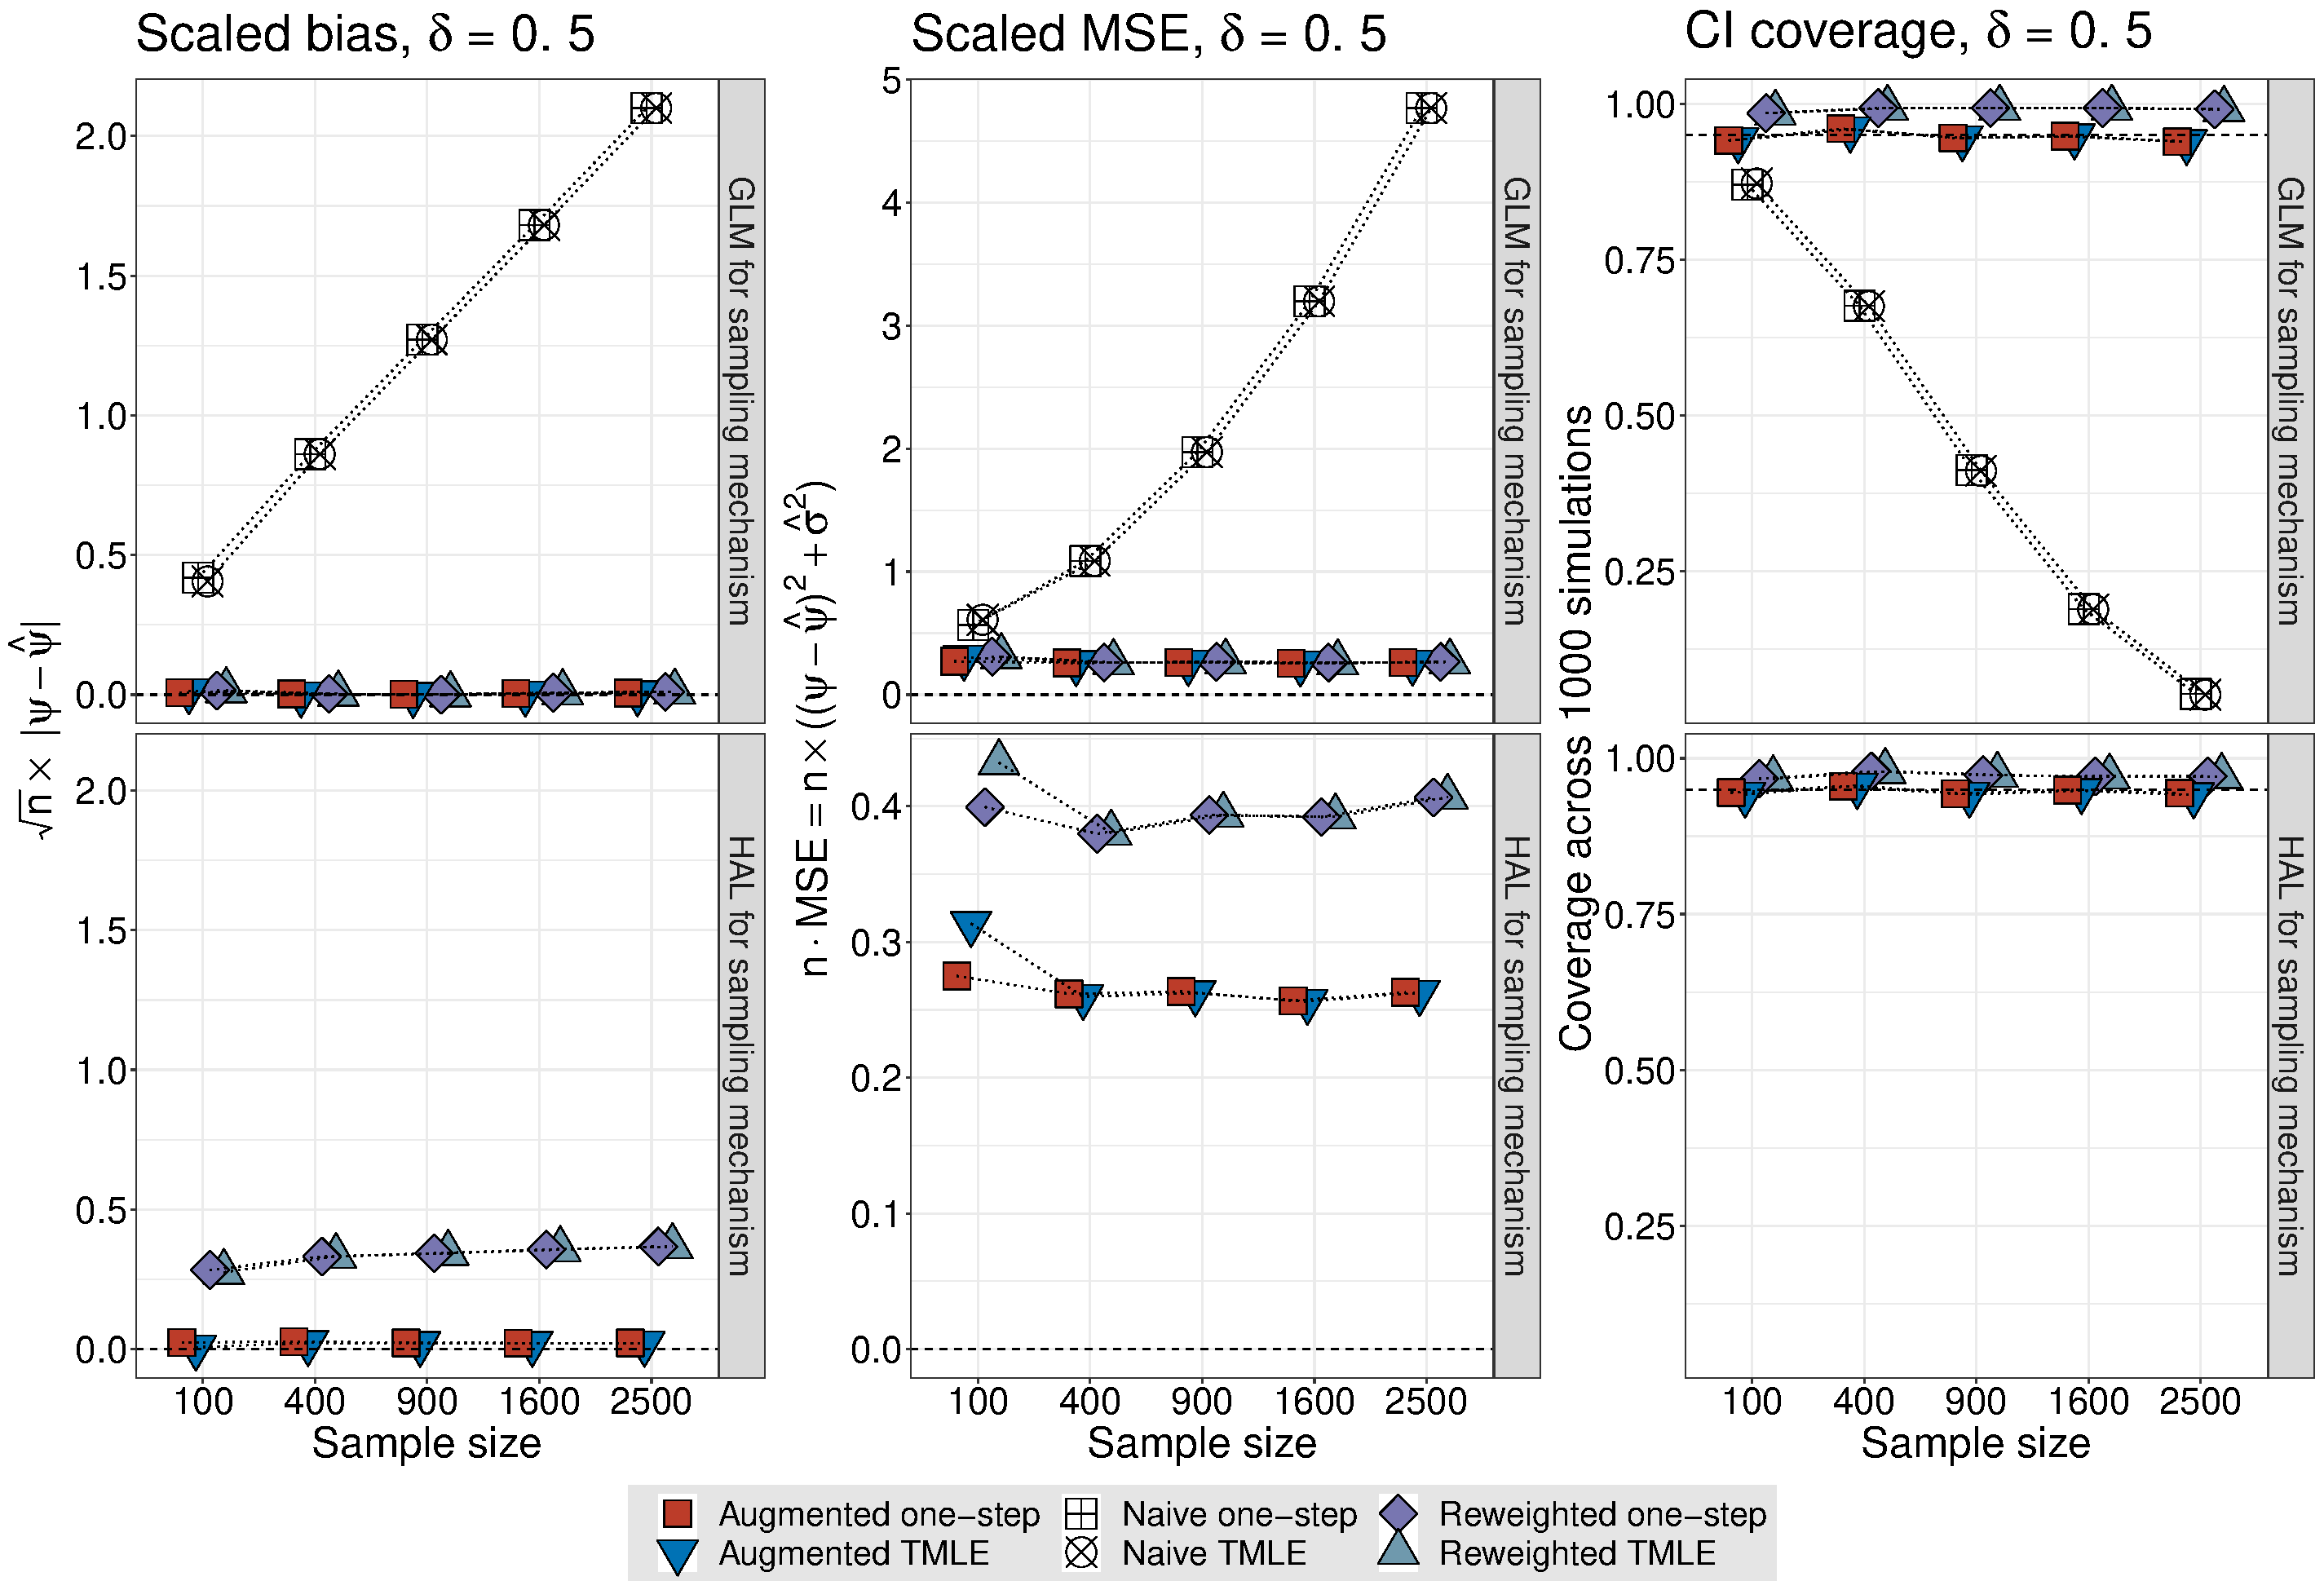
\includegraphics[scale=0.35]{simple_effect_panel_delta_upshift}
  \caption{Comparison of six estimation strategies
  for $\psi_{0,\delta}$ for $\delta = 0.5$, across 1000 Monte Carlo simulations
  for each of five sample sizes. The naive estimators do not make use of the
  estimated sampling mechanism $g_{n,C}$, so their performance is displayed
  only in the upper panel, in the interest of visual economy. This figure
  appears in color in the electronic version of this article, and any mention
  of color refers to that version.}
  \label{fig:simple_sim_delta_upshift}
\end{figure}

When the sampling mechanism is estimated via a correctly specified parametric
model (upper panel), the reweighted and our proposed estimators behave as
expected, with low bias and stable MSE. However, the reweighted estimators
display coverage exceeding 95\%, while our proposed estimators achieve nominal
coverage. This occurs because the influence function that is basis for the
standard error estimates does not include a first-order contribution resulting
from estimation of the sampling mechanism resulting in a conservative standard
error estimate. Unsurprisingly, the naive estimator performed poorly in all
sample sizes, highlighting the importance of accounting for sampling design.

When the sampling mechanism was estimated using HAL (lower panel), the
reweighted estimators do not attain asymptotic linearity, as evidenced by the
scaled bias and MSE increasing with sample size. On the other hand our proposed
estimators have small bias and MSE approaching the efficiency bound, thus
demonstrating the benefits of the additional effort required to produce our
estimators over the simpler reweighted estimators.

Our second simulation study (Section~\ref{sm}) showed that the
efficient estimators provide reliable performance in a setting similar to HVTN
505. Importantly, this setting incorporates both continuous and binary baseline
covariates and a rare outcome ($\approx$5\% incidence). We examine the
performance of our proposed one-step and TML estimators at a sample size of $n
= 1400$ across $\delta \in \{-2, -1.5, -1, 0.5, 0, 0.5, 1, 2\}$ and all nuisance
parameters were estimated via HAL. We found that the proposed estimators achieve
low bias and MSE, as well as empirical coverage of confidence intervals near the
nominal rate. Overall, the TML estimator had slightly better performance than
the one-step estimator.

\section{Application to the HVTN 505 Trial}\label{application}

HVTN 505 enrolled $2504$ HIV-negative participants and randomized participants
1-to-1 to receive an active vaccine or placebo. The one-year incidence of HIV-1
infection was about 1.8\% per person-year in the vaccine arm and 1.4\% per
person-year in the placebo arm, during primary follow-up for HIV-1 acquisition
(between week 28 and month 24; the same period as was used for assessment of
immune correlates). Blood was drawn at the week 26 visit and immune responses
measured for all HIV-1 cases diagnosed between week 28 and month 24 and
a stratified random sample of uninfected controls~\citep{janes2017higher}. The
two-phase sampling of vaccine-recipient controls sampled five controls per case
without-replacement within each of eight baseline covariate strata defined by
categories of body mass index and race/ethnicity (White, Hispanic, Black).
\citet{janes2017higher} and \citet{fong2018modification} analyzed these immune
responses, and both found CD4+ and CD8+ polyfunctionality scores to be
associated with risk of HIV-1 infection status by month 24.

We examined how a range of posited shifts in standardized polyfunctionality
scores of the CD4+ and CD8+ immune markers ($A$) would impact the mean
counterfactual risk of HIV-1 infection ($Y$) in vaccine recipients. We
considered \textit{standardized} polyfunctionality scores, so that our
pre-specified grid of shifts $\delta \in \{-2.0, -1.5, -1.0, -0.5, \allowbreak
0.0, 0.5, 1.0, 1.5, 2.0\}$ can be interpreted as shifts on the standard
deviation (sd) scale. We present results based on our TML estimator; results for
the one-step estimator were similar. To summarize the relationship between the
mean counterfactual risk of HIV-1 infection and shifts in polyfunctionality
scores, a working marginal structural model (MSM) was constructed, as detailed
in section~\ref{msm_summary} of Section~\ref{sm}. Our
augmented TML estimator $\psi_{n,\delta}^{\star}$ requires the construction of
initial estimators of all nuisance functions.

The conditional probability of inclusion in the second-phase sample was
estimated using HAL, adjusting for age, sex, race/ethnicity, body mass index,
and a behavioral risk score for HIV-1 infection. The density $q_{n,A}$ of the
CD4+ or CD8+ polyfunctionality scores ($A$), conditional on the same set of
covariates ($W$), was estimated using our proposed HAL-based conditional density
estimator. The outcome regression $\overline{Q}_{0,Y}$, which estimated the risk
of HIV-1 infection by 24 months ($Y$) given polyfunctionality score and baseline
covariates, was estimated using super learner~\citep{vdl2007super} (details in
Section~\ref{sm}). The pseudo-outcome regression, $G_n$, was
fit via HAL.

Results of applying our estimation procedure separately to both the CD4+ and
CD8+ polyfunctionality scores are presented in
Figure~\ref{fig:hvtn505_tmle_msm}.

\begin{figure}[H]
  \begin{subfigure}{0.9\textwidth}
  \centering
  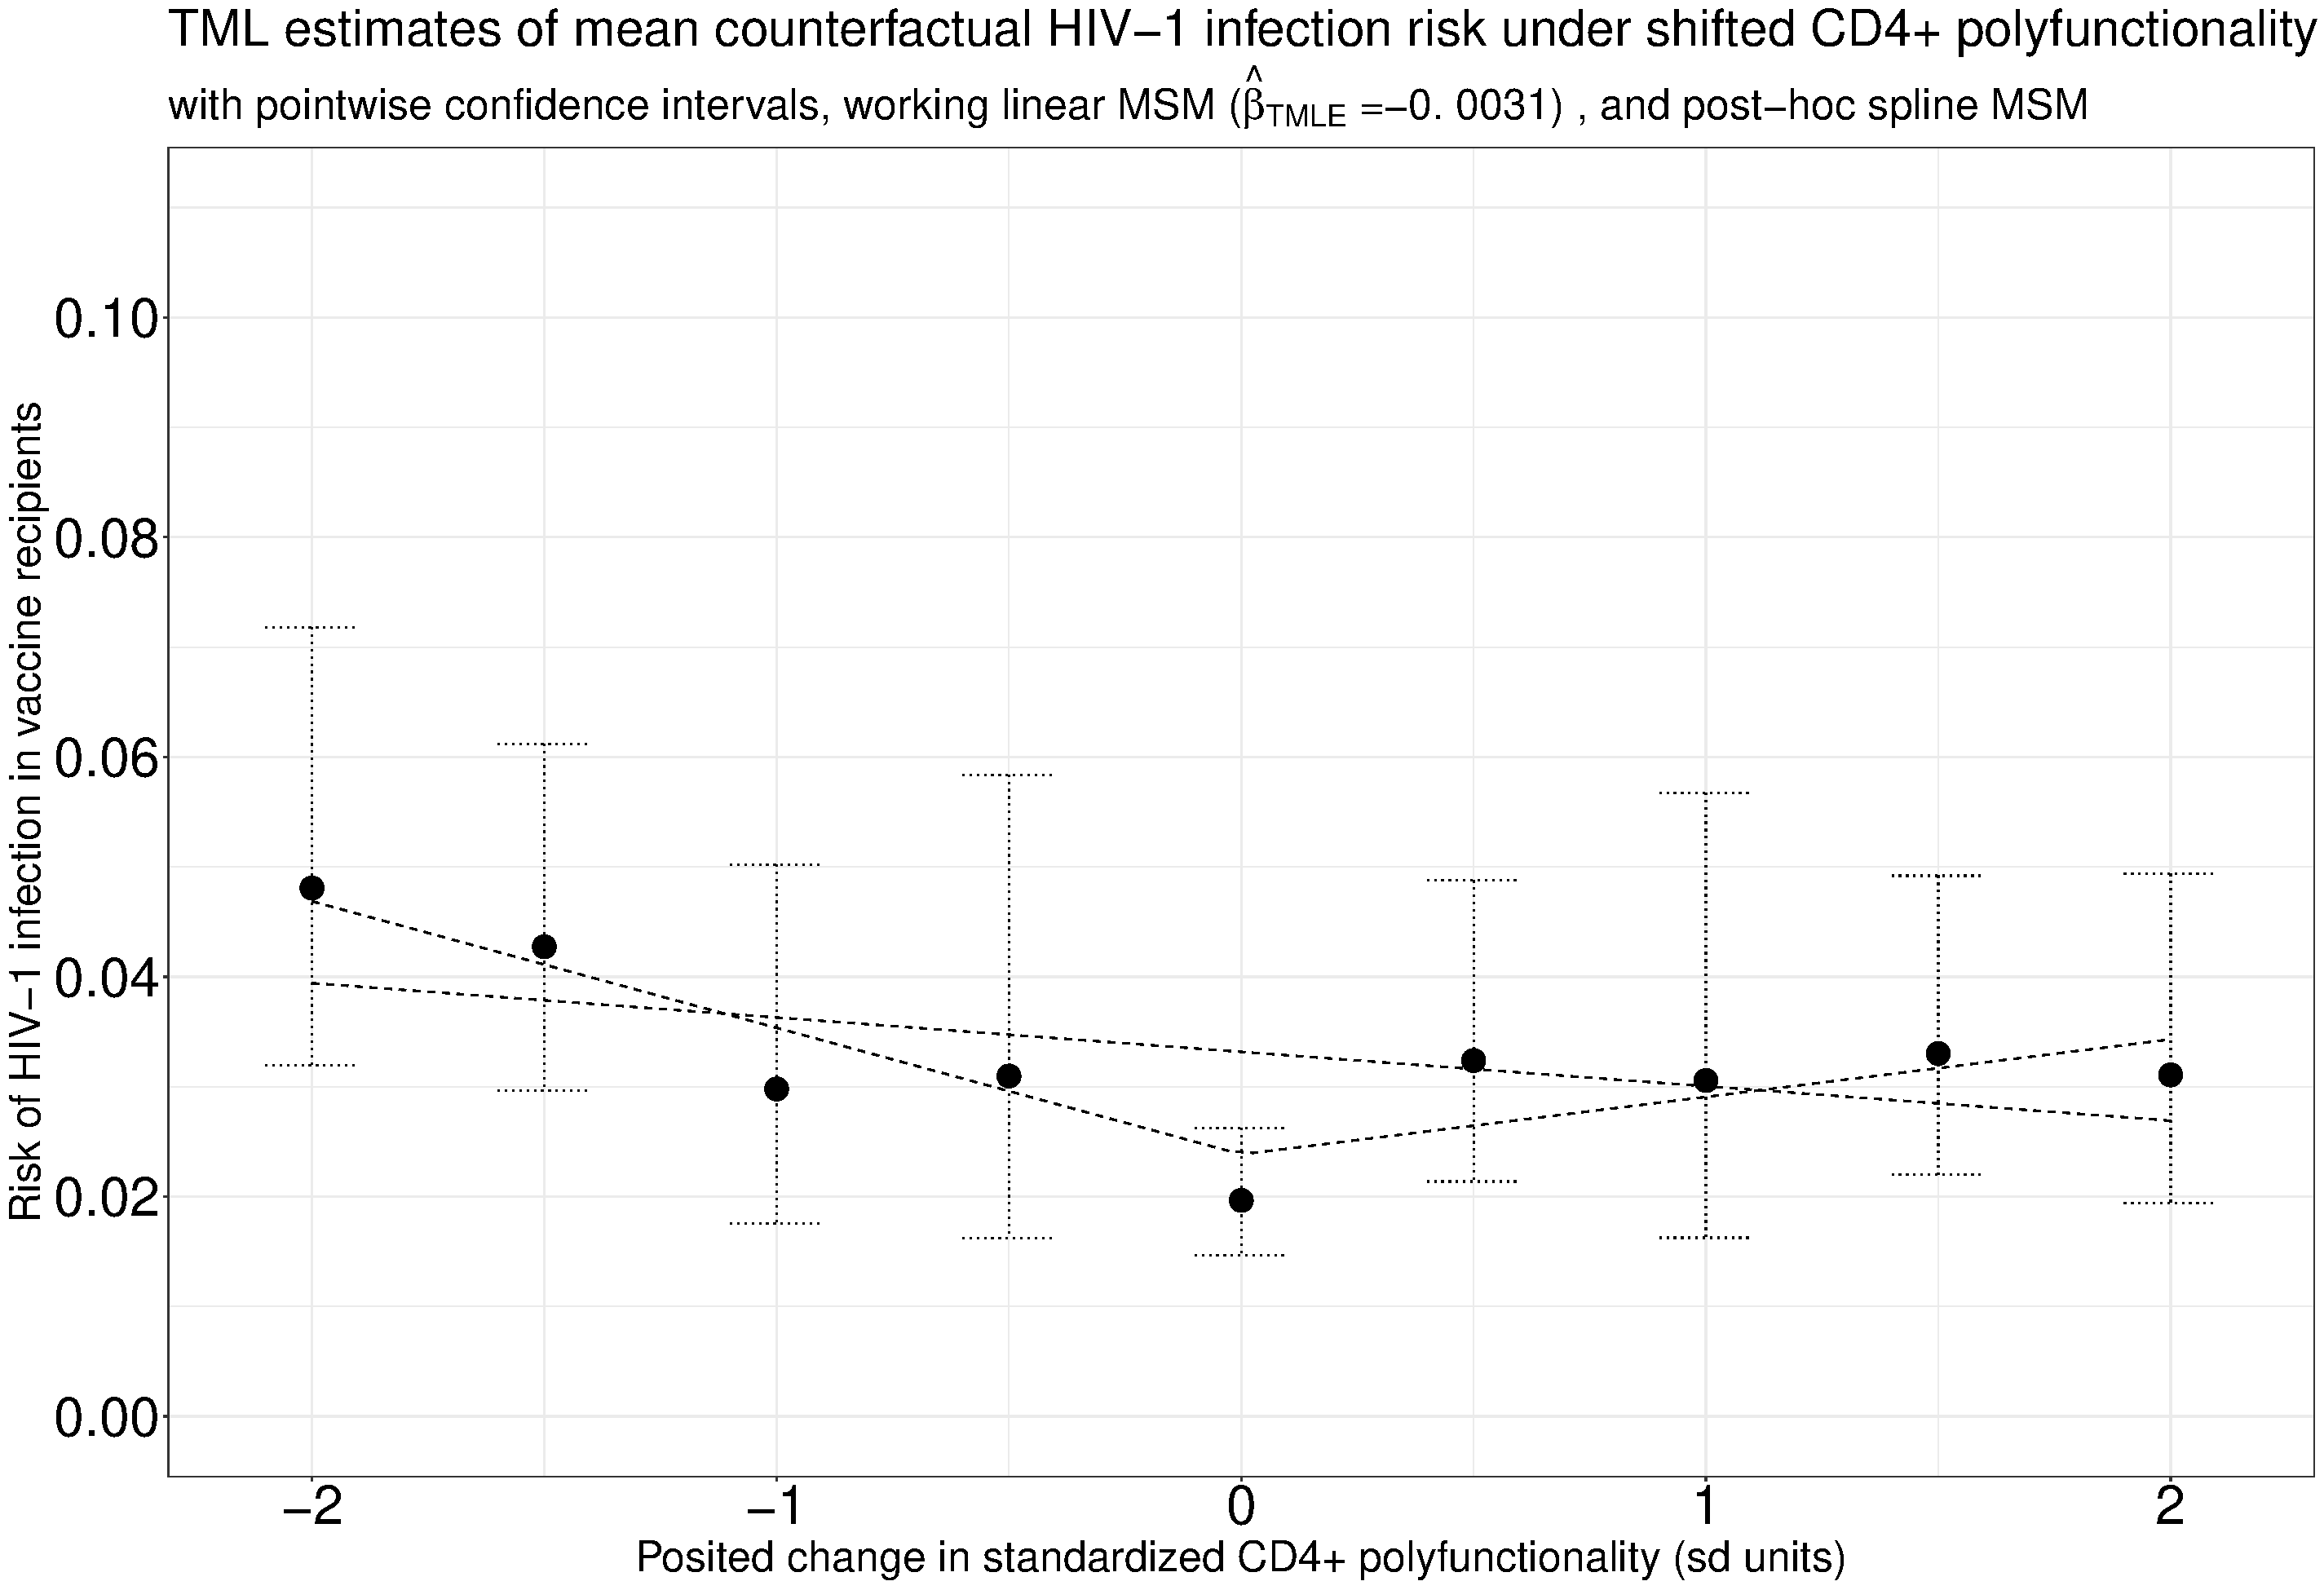
\includegraphics[scale=0.3]{cd4_msm_tmle_summary}
  \label{fig:cd4_tmle_msm}
  \end{subfigure}\\[0.5cm]
  \begin{subfigure}{0.9\textwidth}
  \centering
  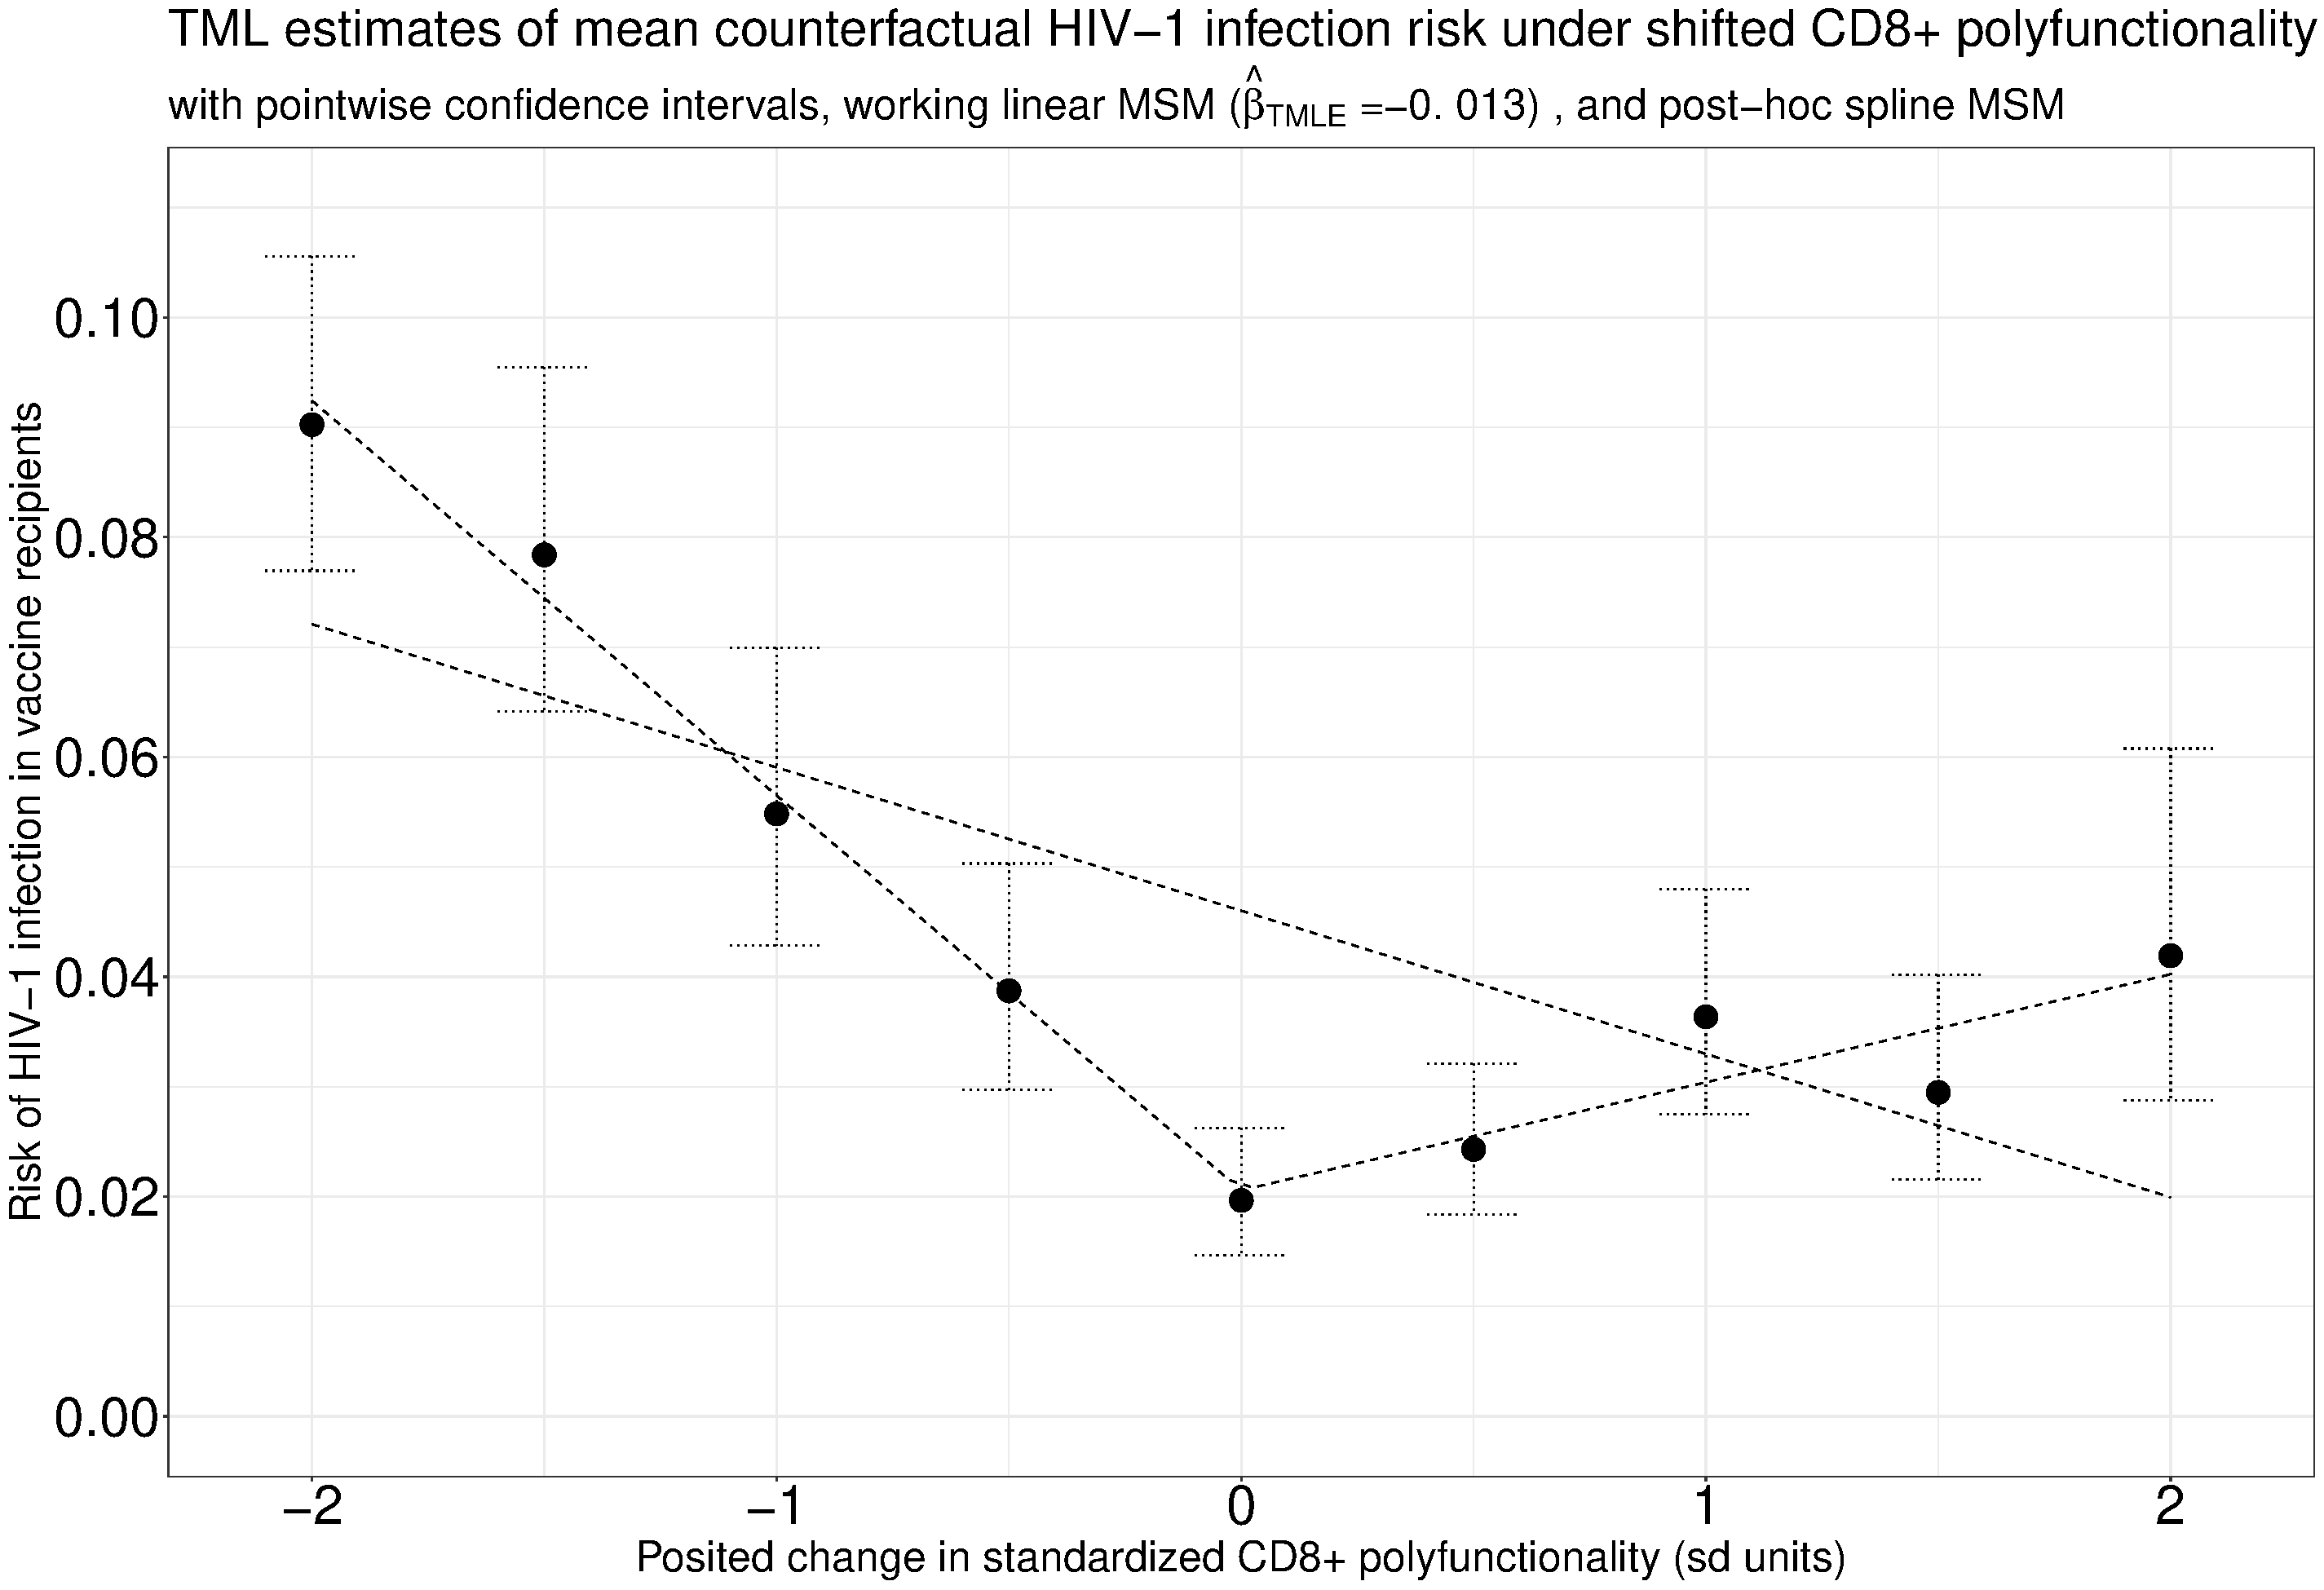
\includegraphics[origin=c,scale=0.3]{cd8_msm_tmle_summary}
  \label{fig:cd8_tmle_msm}
  \end{subfigure}
  \caption{TML estimates of counterfactual HIV-1 infection risk in vaccinees
    under stochastic interventions on CD4+ (top) and CD8+ (bottom) standardized
    polyfunctionality scores. An \textit{a priori} linear working MSM, with
    estimated slope $\hat{\beta}_{\text{TMLE}}$, summarizes the effect of
    shifting the polyfunctionality scores on the HIV-1 infection risk.
    A V-shaped spline model was constructed post-hoc to trace the profile of
    counterfactual HIV-1 risk changes in $\delta$.}
  \label{fig:hvtn505_tmle_msm}
\end{figure}

Examination of the point estimates and confidence intervals of $\psi_{0,\delta}$
in Figure~\ref{fig:hvtn505_tmle_msm} reveals that downshifts in the CD4+
polyfunctionality score led to a small increase in estimated HIV-1 infection
risk among vaccine recipients (Figure~\ref{fig:hvtn505_tmle_msm}, top panel).
For example, examining the individual point estimates, a shift of two standard
units lower in the CD4+ polyfunctionality score was found to at least double the
counterfactual risk of HIV-1 infection. The estimated slope parameter of the
working MSM $\hat{\beta}_{\text{TMLE}}$ pointed to an estimated decrease in risk
of about -0.3\% per standard unit of CD4+ polyfunctionality change.

The estimated result of shifts in the polyfunctionality score of the CD8+
immunological marker displayed a markedly stronger relationship with the risk of
HIV-1 infection (Figure~\ref{fig:hvtn505_tmle_msm}, lower panel). Positive
shifts of the standardized CD8+ polyfunctionality score beyond those observed in
the trial do not appear to have a strong effect on HIV-1 infection risk;
confidence intervals for counterfactual risk estimates for all $\delta \geq 0$
overlap. On the other hand, shifts that lower the CD8+ polyfunctionality score
display a negative linear trend; moreover, confidence intervals for HIV-1 risk
estimates at all $\delta < 0$ do not overlap with those of the estimate at
$\delta = 0$. While this may be taken to indicate that decreases in CD8+ marker
activity adversely affect the risk of HIV-1 infection, we note that this
evidence should be weighed against the fact that all point estimates for
$\delta \neq 0$ are, in fact, higher than that at $\delta = 0$; thus, an
abundance of caution is warranted in drawing conclusions as to whether shifted
CD8+ polyfunctionality score would have improved the HVTN 505 vaccine. Still, it
may be informative that the counterfactual HIV-1 infection risk is over four
times that observed in the HVTN 505 trial at the largest negative shift
considered.
%that is, a vaccine inducing a significantly attenuated immune
%response would have been far less efficacious, underscoring the importance of
%post-vaccination immune response mechanisms in the infection process.

Overall, the results of our analyses support the conclusions of
\citet{janes2017higher} and \citet{fong2018modification}, further indicating
that modulation of the CD4+ and CD8+ polyfunctionality scores may reduce the
risk of HIV-1 infection, with CD8+ polyfunctionality playing a particularly
important role. Notably, our analysis differs from the previous efforts in two
ways: our estimates (i) are based on a formal causal model, which provides an
alternative estimand to summarize relationships between immunogenic response and
risk of HIV-1 infection, and (ii) leverage  machine learning to allow the use of
flexible modeling strategies while simultaneously delivering robust inference.

\section{Discussion}\label{discuss}

A possible criticism of our approach is that, in the context of vaccines, the
immune responses we consider may not be directly manipulable. Nevertheless, we
believe the estimands that we consider pass the important litmus test question:
``If we knew the value of the estimand, could we do something useful with it to
advance science?''~\citep{gilbert2011commentary}. Knowledge of which immune
responses may lead to the largest decrease in infection or disease incidence
would advance vaccine science and stimulate new ideas for the next generation of
vaccine research. Another challenge associated with our approach, as with many
examples in causal inference, is selecting a scientifically meaningful
intervention (i.e., modification of the exposure distribution). While we focused
here on additive shifts for simplicity, more scrutiny of this choice is
warranted in practice. Scientific context could provide some clues as to
potentially meaningful shifts. For example, in the context of influenza
vaccination, past studies have shown that repeated vaccinations may have
a dulling effect on immune responses to new
vaccines~\citep{thompson2016effects}. When such covariate data are available,
they could be used to define an appropriate shift, where the proposed shift is
lessened for individuals with many prior vaccinations.

Our analysis of the HVTN 505 trial could be improved in several respects. First,
there was participant dropout observed in the trial, which our analysis ignored.
A more robust analysis could leverage available covariate information to account
for potentially informative missingness. Further, while we investigate the
effect of altering post-vaccination immune responses on HIV-1 infection, the
issue of interference could limit identifiability of our target causal effects.
In trials conducted across geographically diverse sites or within short time
frames, it may be reasonable to assume that the potential protection conferred
by immune response in a given unit would not alter the infection process in
another unit, satisfying the lack of interference requirement for
identifiability of the causal parameter of interest. Indeed, there is a growing
body of work on relaxing this condition in causal
inference~\citep[e.g.,][]{hudgens2008toward}.

Beyond this issue, there are several other directions for potentially
interesting extensions. First, when a range of shifts is of interest as in our
example, we summarized linear trends using working marginal structural models.
An alternative formulation could examine the stronger null hypothesis that $H_0:
\E Y_{\delta} = \E Y$, uniformly in $\delta$. This is analogous to the
hypothesis tests of~\citet{kennedy2019nonparametric}, which deals with shifted
binary exposure distributions. There, the authors propose a test of this strong
null hypothesis and describe methods for obtaining simultaneous confidence bands
using the multiplier bootstrap. Second, it is of interest to extend our
estimation strategy to other effects based on stochastic interventions, such as
the population intervention (in)direct effects~\citep{diaz2020causal}. Extending
our estimation strategy to such settings and its application in analyzing other
vaccine efficacy trials will be the subject of future research.

\section{Supplementary Materials}\label{sm}

While no new data were generated or analyzed in the present work, the results of
our reported analyses may be reproduced using the publicly available \texttt{R}
code at \url{https://github.com/nhejazi/pub_txshift_biometrics}. Throughout our
simulation experiments and data analyses, we rely on our \texttt{txshift} and
\texttt{haldensify} \texttt{R} packages, available at
\url{https://github.com/nhejazi/txshift} and
\url{https://CRAN.R-project.org/package=haldensify}, respectively. The
\texttt{txshift} \texttt{R} package implements our proposed efficient estimators
of the counterfactual mean outcome under a stochastic intervention, while our
\texttt{haldensify} \texttt{R} package provides a nonparametric estimator of the
generalized propensity score.

\subsection{Conditional density estimation based on the highly adaptive
lasso}\label{cond_dens}

In section~\ref{est_nuisance_param}, several of the challenges associated
with conditional density estimation were briefly expressed. The auxiliary
covariate appearing in the form of the EIF is a ratio of such conditional
densities. In the construction of our proposed estimators, the exposure
mechanism $q_{0,A}$ is a density of the intervention $A$, conditional on the
observed covariates $W$, which must be evaluated at both the observed values and
the post-intervention counterfactual values. As consistent estimation of the the
generalized propensity score is an integral part of our proposed methodology, we
outline here a conditional density estimator, built around the HAL regression
function, that achieves the convergence rate required by our formal theorem. We
note that proposals for the data adaptive estimation of such quantities are
sparse in the literature~\citep[e.g.,][]{zhu2015boosting}. Notably,
\citet{diaz2011super} gave a proposal for constructing semiparametric estimators
of such a target quantity based on exploiting the relationship between the
hazard and density functions. Our proposal builds upon theirs in several key
ways: (i) we adjust their algorithm so as to incorporate sample-level weights,
necessary for making use of inverse probability of censoring weights; and (ii)
we replace their use of an arbitrary classification model with one based on the
HAL regression function. While our first modification is general and may be
applied to the estimation strategy \citet{diaz2011super} propose, our latter
contribution requires adjusting the penalization aspect of HAL regression to
respect the use of a loss function appropriate for prediction on the hazard
scale. To make these contributions widely accessible, we introduce the
\texttt{haldensify} \texttt{R} package~\citep{hejazi2020haldensify}, available
at \url{https://github.com/nhejazi/haldensify}

To build an estimator of a conditional density, \citet{diaz2011super} considered
discretizing the observed $a \in A$ based on a number of bins $T$ and a binning
procedure (e.g., including the same number of points in each bin or forcing
bins to be of the same length). We note that the choice of the tuning parameter
$T$ corresponds roughly to the choice of bandwidth in classical kernel density
estimation; this will be made clear upon further examination of the proposed
algorithm. The data $\{A, W\}$ are reformatted such that the hazard of an
observed value $a \in A$ falling in a given bin may be evaluated via standard
classification techniques. In fact, this proposal may be viewed as
a re-formulation of the classification problem into a corresponding set of
hazard regressions:
$\prob (a \in [\alpha_{t-1}, \alpha_t) \mid W) = \prob (a \in [\alpha_{t-1},
\alpha_t) \mid A \geq \alpha_{t-1}, W) \times \prod_{j = 1}^{t -1} \{1 - \prob
(a \in [\alpha_{j-1}, \alpha_j) \mid A \geq \alpha_{j-1}, W) \}$,
where the probability that a value of $a \in A$ falls in a bin $[\alpha_{t-1},
\alpha_t)$ may be directly estimated from a standard classification model. The
likelihood of this model may be re-expressed in terms of the likelihood of
a binary variable in a data set expressed through a repeated measures structure.
Specifically, this re-formatting procedure is carried out by creating a data set
in which any given observation $A_i$ appears (repeatedly) for as many intervals
$[\alpha_{t-1}, \alpha_t)$ that there are prior to the interval to which the
observed $a$ belongs. A new binary outcome variable, indicating $A_i \in
[\alpha_{t-1}, \alpha_t)$, is recorded as part of this new data structure. With
the re-formatted data, a pooled hazard regression, spanning the support of $A$
is then executed. Finally, the conditional density estimator
$q_{n, \alpha}(a \mid W) = (\prob(a \in [\alpha_{t-1}, \alpha_t) \mid W)) /
(\alpha_t - \alpha_{t-1})$,
for $\alpha_{t-1} \leq a < \alpha_t$, may be constructed. As part of this
procedure, the hazard estimates are mapped to density estimates through
rescaling of the estimates by the bin size ($\alpha_t - \alpha_{t-1}$).

In its original proposal, a key element of this procedure was the use of any
arbitrary classification procedure for estimating $\prob(a \in [\alpha_{t-1},
\alpha_t) \mid W)$, facilitating the incorporation of flexible, data adaptive
estimators. We alter this proposal in two ways, (i) replacing the arbitrary
estimator of $\prob(a \in [\alpha_{t-1}, \alpha_t) \mid W)$ with HAL regression
and (ii) accommodating the use of sample-level weights, making it possible for
the resultant conditional density estimator to achieve a convergence rate with
respect to a loss-based dissimilarity of $n^{-1/4}$ under only mild assumptions.
This is an important advance that is needed for the asymptotic analysis of our
proposed estimators, as per section~\ref{asymp_analy}. As a secondary
advance, our procedure alters the HAL regression function to use a loss function
tailored for estimation of the hazard, invoking $\ell_1$-penalization in
a manner consistent with this loss.

\subsection{Algorithm for efficient targeted minimum loss
  estimation}\label{tmle_algo}

In section~\ref{os_tml_est}, we introduced a novel algorithm for targeted
minimum loss estimation with inverse probability of censoring weights. We
formalize our procedure in Algorithm~\ref{alg:ipcw_targeting}:

\begin{algorithm}[H]
\label{alg:ipcw_targeting}
\SetAlgoLined
\KwResult{Updated sampling mechanism estimate $g_{n,C}^{\star}$ and updated
  outcome mechanism estimate $\overline{Q}_{n,Y}^{\star}$}
\SetKwInOut{Input}{Input}\SetKwInOut{Output}{Output}
\Input{
  \begin{itemize}
    \item[] Initial estimate of the sampling mechanism: $g_{n,C} \in [0, 1]$
    \item[] Initial estimate of the outcome mechanism: $\overline{Q}_{n,Y}
        \in \R$
    \item[] Estimate of the EIF pseudo-outcome regression: $G_n \in \R$
    \item[] Estimate of the auxiliary covariate of the EIF: $H_n \in \R$
    \item[] Observed indicators of the sampling mechanism: $C \in \{0, 1\}$
  \end{itemize}
}
\BlankLine
Initialize $g_{n,C}^{\star} \coloneqq 0$ and
$\overline{Q}_{n,Y}^{\star} \coloneqq 0$\;
\BlankLine
\While{$g_{n,C}^{\star} = 0$ and $\overline{Q}_{n,Y}^{\star} = 0$}{
Define a working logistic regression model $\logit(g_{n, C, \xi}) =
     \logit(g_{n,C}) + \xi (G_n / g_{n,C}) : \xi \in \R$ and evaluate the MLE
     $\xi_n$ of the parameter $\xi$, e.g., via iteratively reweighted least
     squares\;
With the MLE $\xi_n$, extract predictions from this working model for
    the outcome, the conditional mean of $C$ given $\{Y, W\}$, constructing the
    updated estimate $g_{n,C}^{\star} \coloneqq g_{n, C, \xi_n}$\;
Define a weighted working logistic regression model
    $\logit(\overline{Q}_{n, Y, \epsilon}) = \logit(\overline{Q}_{n,Y}) +
    \epsilon H_n : \epsilon \in \mathbb{R}$, with weights $C_i
    / g^{\star}_{n,C}(Y_i,W_i)$, and construct the MLE
    $\epsilon_n$ of the model parameter $\epsilon$\;
With the MLE $\epsilon_n$, construct the updated estimate of the
    outcome, the conditional mean of $Y$ given $\{A,W\}$, by prediction to
    obtain $\overline{Q}_{n,Y}^{\star} \coloneqq \overline{Q}_{n, Y,
    \epsilon_n}$.
}
\BlankLine
\Output{
  \begin{itemize}
    \item[] $g_{n,C}^{\star}$, an updated estimate of the sampling mechanism.
     \item[] $\overline{Q}_{n,Y}^{\star}$, an updated estimate of the outcome
       mechanism.
  \end{itemize}
}
\caption{Efficient updating procedure for IPCW-TML estimation}
\end{algorithm}

Note that in the two working logistic regression models defined above, the
inputs $g_{n,C}$ and $\overline{Q}_{n,Y}$ are both treated as offsets (known
parameter value equal to one); thus, the working models are one-dimensional.

The outlined procedure includes two targeting steps. The first of these steps
constructs an update of the initial estimator of the second-phase sampling
probability, $g_{n,C}^{\star}$, based on the initial estimate of $G_n$. This
step ensures that the revised estimate satisfies $\sum_{i=1}^n \{G_n(Y_i, W_i)
/ g_{n,C}^{\star}(Y_i,W_i\} \{C_i - g_{n,C}^{\star}(Y_i, W_i)\} = 0$. in
a single step when a universal least favorable submodel~\citep{vdl2016one} is
used, though an iterative procedure based on locally least favorable parametric
submodels may be used to achieve the same result. In the second step, the
updated outcome regression $\overline{Q}_{n,Y}^{\star}$ is generated based on
the conditional density estimate $q_{n,A}$; the inclusion of weights in the
regression ensures that $\sum_{i=1}^n C_i/g_{n,C}(Y_i, W_i) D_{n,i}^F = 0$.

\subsection{Summarization via working marginal structural
models}\label{msm_summary}

%\db{Basically, the point is that $\psi_{0,d}$ is like one
%counterfactual mean. So I can know the mean if I give everyone treatment, but
%that's only useful if I also know the mean when every one takes control. So we
%need to make explicit that we're trying to define an interesting
%\textit{contrast}.}
Estimation of $\psi_{0,\delta}$ for a single pre-specified shift $\delta$ may be
unsatisfactory in some contexts, as it does not provide information concerning
a dose-response relationship between exposure and outcome. Thus, to develop an
understanding of a dose-response pattern in the context of stochastic
interventions, it may be informative to estimate the counterfactual mean outcome
across several values of $\delta$. In the context of HVTN 505, we consider
estimation of a grid of counterfactual means $\psi_0 = (\psi_{n,\delta_1},
\ldots, \psi_{n,\delta_K})$ and examine how the risk of HIV infection varies
with choice of $\delta$ over a fixed grid, i.e., $\delta_k \in \{\delta_1,
\ldots, \delta_K\}$. After estimating the counterfactual mean for each
$\delta_k$, a summary measure relating the stochastic
interventions to the mean counterfactual outcomes may be constructed by
projection onto a working marginal structural model (MSM). For example, we might
consider a (possibly weighted) least-squares projection on the linear working
model $m_{\beta}(\delta) = \beta_0 + \beta_1 \delta$, in which case the
parameter $\beta_1$ corresponds to the linear trend in mean counterfactual
outcomes as a function of the $\delta_k$.

More generally, we can define $\beta(\delta)=\argmin_{\beta \in \mathbb{R}^d}
\sum_{\delta \in \{\delta_1, \ldots, \delta_K\}} h(\delta)\{\psi_{0,\delta}
- m_{\beta}(\delta)\}^2$, for a user-selected weight function $h(\delta)$. We
note that adjustment of the weight function, as well as the functional form of
$m_{\beta}(\delta)$, allow for a wide variety of working models to be
considered. Alternatively, $\beta(\delta)$ can be viewed as the solution of
\begin{equation*}
  0 = U(\beta,\psi) = \sum_{\delta \in \{\delta_1, \ldots, \delta_K\}}
  h(\delta) \frac{d}{d\beta} m_{\beta}(\delta) \{\psi_{0,\delta} -
  m_{\beta}(\delta)\}.
\end{equation*}
The goal is to make statistical inference on the parameter $\beta$. We note that
this approach does not assume a linear dose-response curve, but rather uses
a working model to summarize the relationship between exposure and outcome
\citep{neugebauer2007nonparametric}. This approach is distinct from that of
\citet{haneuse2013estimation}, whose proposal involving MSMs pertains
specifically to parametric models.

To estimate $\beta$, we assume access to the TML or one-step estimates $\psi_n
= (\psi_{n, \delta_1}, \ldots, \psi_{n,\delta_K})$ for each $\delta_k$. The
estimate $\beta_n$ of $\beta$ is the solution in $\beta$ of the equation $0
= U(\beta,\psi_n)$. To derive the limit distribution of $\beta_n$, let
$D_{0,\psi}$ denote a vector whose $k^{\text{th}}$ entry is the EIF associated
with parameter $\psi_{0,\delta_k}$. The delta method implies that the influence
function of $\beta_n$ is $D_{\beta} = [-\frac{d}{d \beta} U(\beta,\psi_0)^{-1}]
\frac{d}{d\psi_0} U(\beta, \psi_0) D_{\psi_0}$, and that $n^{1/2} (\beta_n
- \beta)$ converges in distribution to a mean-zero Gaussian random variable with
variance $\Sigma = \E_{P_0}\{D_{\beta}(O)^2\}$. The empirical covariance matrix
of $D_{0,\psi}$ evaluated at nuisance parameter estimates serves to estimate
$\Sigma$.

%\vdl{define $\beta(\delta)=\argmin_{\beta} \sum_{\delta}
%h(\delta)(\psi(\delta) - m_{\beta}(\delta))^2$ that solves
%$0=U(\beta,\psi) = \sum_{\delta} h(\delta) \frac{d}{d\beta} m(\psi(\delta) -
%m_{\beta}(\delta))$. This equation defines $\beta=\beta(\psi)$ as function of
%$\psi$-vector. The implicit function theorem says $\frac{d}{d \psi} \beta(\psi)
%= [-\frac{d}{d \beta} U(\beta, \psi)^{-1}] \frac{d}{d \psi} U(\beta,\psi)$ so
%$D_{\beta}=[-\frac{d}{d \beta} U(\beta,\psi)^{-1}] \frac{d}{d \psi}
%U(\beta,\psi) D_{\psi}$ (the last one is gradient on its side), where
%$D_{\psi}$ is vector efficient influence function of $\psi$ vector. the front
%is your matrix inverse. the last part if the gradient applied to $D_{\psi}$.}

%$\sum_{k = 1}^K h(\delta_k) \left(\psi_{0,\delta_k} -
%m_{\beta}(\delta_k) \right) \frac{d}{d\beta} m_{\beta}(\delta_k) = 0$, where
%$h(\delta)$ is a weight function. To estimate $\beta$ and derive confidence
%intervals and hypothesis tests for $\beta$, we note its EIF $D_{\beta}(O)$ may
%be written in terms of the EIFs $D_{\psi_{0,\delta_k}}(O)$ of the
%$\psi_{0,\delta_k}$ by application of the delta method, yielding
%\begin{equation*}
  %D_{\beta}(O) = \left(\sum_{k=1}^K h(\delta_k) \frac{d}{d\beta}
  %m_{\beta}(\delta_k) \frac{d}{d\beta} m_{\beta}(\delta_k)^T \right)^{-1} \cdot
  %\sum_{k=1}^K h(\delta_k) \frac{d}{d\beta} m_{\beta}(\delta_k)
  %D_{\psi_{0,\delta_k}}(O).
%\end{equation*}
%Substituting the linear working MSM for an analogous generalized linear model
%allows this projection approach to be applied to arbitrary finite-dimensional
%regression models.

%\db{I couldn't really follow this math. What is $h$? I would just show the math
%explicitly for the linear regression example (i.e., show how to compute
%estimators, get standard error estimates, build confidence intervals), and just
%state that the ideas generalize the projections onto arbitrary
%finite-dimensional regression models.}
%we note the first-order
%expansion $\beta(\widetilde{\psi}_{n,d}) - \beta(\widetilde{\psi}_{0,d}) \approx
%- \frac{d}{d\beta} u(\beta_0, \widetilde{\psi}_{0,d})^{-1} \frac{d}{d\psi}
%u(\beta_0, \psi_0)(\widetilde{\psi}_{n,d} - \widetilde{\psi}_{0,d})$, where
%where we have
%$\frac{d}{d\beta} u(\beta, \psi) = -\sum_{\delta} h(\delta) \frac{d}{d\beta}
%m_{\beta}(\delta)^t \frac{d}{d\beta} m_{\beta}(\delta),$
%and $\frac{d}{d\psi}u(\beta, \psi)(\psi_n - \psi_0) = \sum_{\delta} h(\delta)
%\frac{d}{d\beta} m_{\beta}(\delta) (\psi_n - \psi_0)(\delta)$.

\subsection{Proof of Theorem~\ref{theo:aslintmle}}

We now examine a proof of the theorem establishing conditions for the weak
convergence of our efficient estimators. Building upon
section~\ref{background}, note that the full data parameter may be
expressed as a mapping $\Psi^F: \M^X \rightarrow \R$ and that $\Psi^F(P_0^X)
\equiv \Psi^F(\overline{Q}_{0,Y})$, since the parameter mapping depends on
$P_0^X$ only through the functional $\overline{Q}_{0,Y}$. We recall that the EIF
$D^F(\overline{Q}_{0,Y},g_{0,A})$ coincides with the canonical gradient of the
parameter mapping $\Psi^F: \M^X \rightarrow \R$, since a regular asymptotically
linear estimator with influence function equal to the canonical gradient is
asymptotically efficient~\citep{bickel1993efficient, vdl2003unified}. Note
further that the observed data parameter is defined such that $\Psi(P_0) \equiv
\Psi^F(P^X_0)$, where the observed data parameter mapping $\Psi:\M \rightarrow
\R$ is pathwise differentiable at a distribution $P$ in the statistical model
with a gradient given by the EIF:
\begin{equation*}
  D(G_0, g_{0,C}, D^{F}(\overline{Q}_{0,Y}, q_{0,A}))(o) =
  \frac{C}{g_{0,C}(y, w)} D^F(\overline{Q}_{0,Y}, q_{0,A})(x) -
  \frac{G_0(y,w)}{g_{0,C}(y,w)}(C - g_{0,C}(y,w)) \ .
\end{equation*}
The class of all gradients of $\Psi$ at $P$ is given by $\{D(G_0, g_{0,C},
D^F(P^X)): D^F(P^X)\}$ where $D^F(P^X)$ varies over all gradients of the
full data parameter $\Psi^F$ at distributions $P^X \in \M^X$. As $D^F$ varies,
$G_0$ also necessarily varies since it is defined as the conditional mean of
$D^F$ given $\{C = 1, Y, W\}$. In particular, if the full data model $\M^X$ is
nonparametric, then there is only one full data gradient, which is the canonical
gradient (or EIF) of $\Psi$ at $P$.

In the sequel, let $\lVert f \rVert_2 = \E\{f(O)^2\}^{1/2}$ denote the
$L^2(P_0)$ norm of a $P_0$-measurable function $f$, define $\widetilde{G}_0
\coloneqq \E_{P_0}[D^F(\overline{Q}^{\star}_{n,Y}, q_{n,A})(O) \mid C = 1, Y,
W]$, and let $G_n$ be the estimate of $\widetilde{G}_0$. An exact
characterization of the second-order remainder for the full data parameter
$\Psi^F(P^X) - \Psi^F(P_0^X)$ is given by
\begin{equation*}
  R^F_2(\overline{Q}_{n,Y}, q_{n,A}, \overline{Q}_{0,Y}, q_{0,A}) \coloneqq
    \Psi^F(\overline{Q}_{n,Y})-\Psi^F(\overline{Q}_{0,Y}) +
    \E_{P^X_0}[D^F(\overline{Q}_{n,Y}, q_{n,A})]
\end{equation*}
while the exact second-order remainder for the observed data parameter
$\Psi(P)-\Psi(P_0)$ is analogously defined
\begin{equation*}
  R_2(P, P_0) \coloneqq \Psi(P) - \Psi(P_0) + \E_{P_0}[D(G_n, g_{n,C},
  D^F(\overline{Q}_{n,Y}, q_{n,A}))].
\end{equation*}
Combining these definitions, the exact second-order remainder for the observed
data parameter may be expressed in terms of the second-order remainder of its
full data counterpart:
\begin{equation*}
  R_2(P, P_0) = R_2^F(\overline{Q}_{n,Y}, q_{n,A}, \overline{Q}_{0,Y}, q_{0,A})
    + \E_{P_0} \left[ \left(\frac{g_{n,C} - g_{0,C}}{g_{n,C}} \right) (G_n -
    \widetilde{G}_0) \right].
\end{equation*}

Assume the following conditions:
\begin{assumption}\label{ass:eif_rootn}
  $\E_{P_n} D(G_n, g^{\star}_{n,C}, D^F(\overline{Q}^{\star}_{n,Y},
    q_{n,A})) = 0$.
\end{assumption}
\begin{assumption}\label{ass:sampling_bound}
  $g_{0,C} > \zeta > 0$ and $g^{\star}_{n,C} > \zeta$ with probability tending
  to 1 for some $\zeta > 0$.
\end{assumption}
\begin{assumption}\label{ass:obs_eif_parametric}
    $\lVert G_n - \widetilde{G}_0 \rVert_{P_0} = o_P(n^{-1/4})$ and
        $\lVert g^{\star}_{n,C} - g_{0,C} \rVert_{P_0} = o_P(n^{-1/4})$.
\end{assumption}
\begin{assumption}\label{ass:r2_fulldata}
  $R_2^F(\overline{Q}^{\star}_{n,Y}, q_{n,A}, \overline{Q}_{0,Y},
       q_{0,A}) = o_P(n^{-1/2})$.
\end{assumption}
\begin{assumption}\label{ass:neglig_obs_eif}
   $\lVert D(G_n, g^{\star}_{n,C}, D^F(\overline{Q}^{\star}_{n,Y},
        q_{n,A})) - D(G_0, g_{0,C}, D^{F}(\overline{Q}_{0,Y}, q_{0,A}))
        \rVert_{P_0} = o_P(1)$.
\end{assumption}
\begin{assumption}\label{ass:donsker}
   Let $\mathcal{F}_v^{\star}(M)$ be the class of cadlag functions $f$
   on a cube $[0,\tau] \subset \R^d$ (for some integer $d$), for which the
   sectional variation norm $\lVert f \rVert_v^{\star}$ is bounded by a
   universal constant $M < \infty$. Assume that $D(G_n,
   g^{\star}_{n,C}, D^{F}(\overline{Q}^{\star}_{n,Y}, q_{n,A})) \in
   \mathcal{F}_v^{\star}(M)$ with probability tending to 1 (n.b., the
   definition $\mathcal{F}_v^{\star}(M)$ can be replaced by any Donsker class).
\end{assumption}

\begin{proof}[Theorem~\ref{theo:aslintmle}: asymptotic linearity and
efficiency of the TML estimator $\psi_{n,\delta}^{\star}$]\label{pf:aslintmle}
Under conditions~\ref{ass:eif_rootn}--\ref{ass:donsker}, we have $\E_{P_n}
D(G_n, g^{\star}_{n,C}, D^F(\overline{Q}^{\star}_{n,Y},q_{n,A})) =
o_P(n^{-1/2})$; moreover, by definition of $R_2(P, P_0)$:
\begin{align*}
  \Psi^F(\overline{Q}^{\star}_{n,Y}) - \Psi^F(\overline{Q}_{0,Y}) =
   &-\E_{P_0} [D(G_n, g^{\star}_{n,C},
      D^F(\overline{Q}^{\star}_{n,Y}, q_{n,A}))] \\
   &+ R^F_2(\overline{Q}^{\star}_{n,Y}, q_{n,A}, \overline{Q}_{0,Y}, q_{0,A})
  + \E_{P_0} \left[ \left( \frac{g^{\star}_{n,C} - g_{0,C}}
   {g^{\star}_{n,C}} \right) (G_n - \widetilde{G}_0)\right].
\end{align*}
Combining with condition~\ref{ass:eif_rootn}, we have
\begin{align*}
  \Psi^F(\overline{Q}^{\star}_{n,Y}) - \Psi^F(\overline{Q}_{0,Y}) =
  & \E_{P_n}[D(G_n, g^{\star}_{n,C}, D^F(\overline{Q}^{\star}_{n,Y}, q_{n,A}))]
  - \E_{P_0}[D(G_n, g^{\star}_{n,C}, D^F(\overline{Q}^{\star}_{n,Y},
  q_{n,A}))] \\
  &+ R^F_2(\overline{Q}^{\star}_{n,Y}, q_{n,A}, \overline{Q}_{0,Y}, q_{0,A}) +
  \E_{P_0} \left[ \left( \frac{g^{\star}_{n,C} - g_{0,C}}{g^{\star}_{n,C}}
  \right) (G_n - \widetilde{G}_0) \right]
\end{align*}

The sum of the first two terms equals $\E_{P_n}[D(G_0, g^{\star}_{0,C},
D^F(\overline{Q}^{\star}_{0,Y}, q_{0,A})(O)] + o_{P}(n^{-1/2})$ as implied by
conditions~\ref{ass:neglig_obs_eif} and~\ref{ass:donsker}.
Condition~\ref{ass:r2_fulldata} ensures the third term equals $o_{P}(n^{-1/2})$.
Conditions~\ref{ass:sampling_bound} and~\ref{ass:obs_eif_parametric} imply that
the fourth term equals $o_P(n^{-1/2})$, which completes the proof. An analogous
proof holds for the one-step estimator $\psi_{n,\delta}^{+}$ when the initial
estimates $\overline{Q}_{n,Y}$ and $g_{n,C}$ are used instead of their revised
counterparts. Here, we do not require condition~\ref{ass:eif_rootn}, as our
proposed estimation procedure guarantees that it will be attained.
\end{proof}

\subsection{Results of Additional Simulation Studies}\label{more_sims}

\subsubsection{Simulation \#1b: Comparison of estimator variants under the
  shifts $\delta = -0.5$ and $\delta = 0$}\label{sim1_supp}

In the results reported in section~\ref{sim}, for our first simulation
study under the shift $\delta = 0.5$, we noted excellent performance of our
proposed estimator variants under several standard metrics, including
$\sqrt{n}$-bias, $n$-MSE, and the coverage of confidence intervals. To further
assess the quality of performance of our augmented estimators, we examine the
same six estimator variants under the shifts $\delta \in \{-0.5, 0\}$. Details
of the simulation study have been previously described in
section~\ref{sim}. As before, results are reported based on aggregation
across $1000$ repetitions. The results of these numerical investigations are
reported in Figures~\ref{fig:simple_sim_delta_noshift}
and~\ref{fig:simple_sim_delta_downshift}.

\begin{figure}[H]
  \centering
  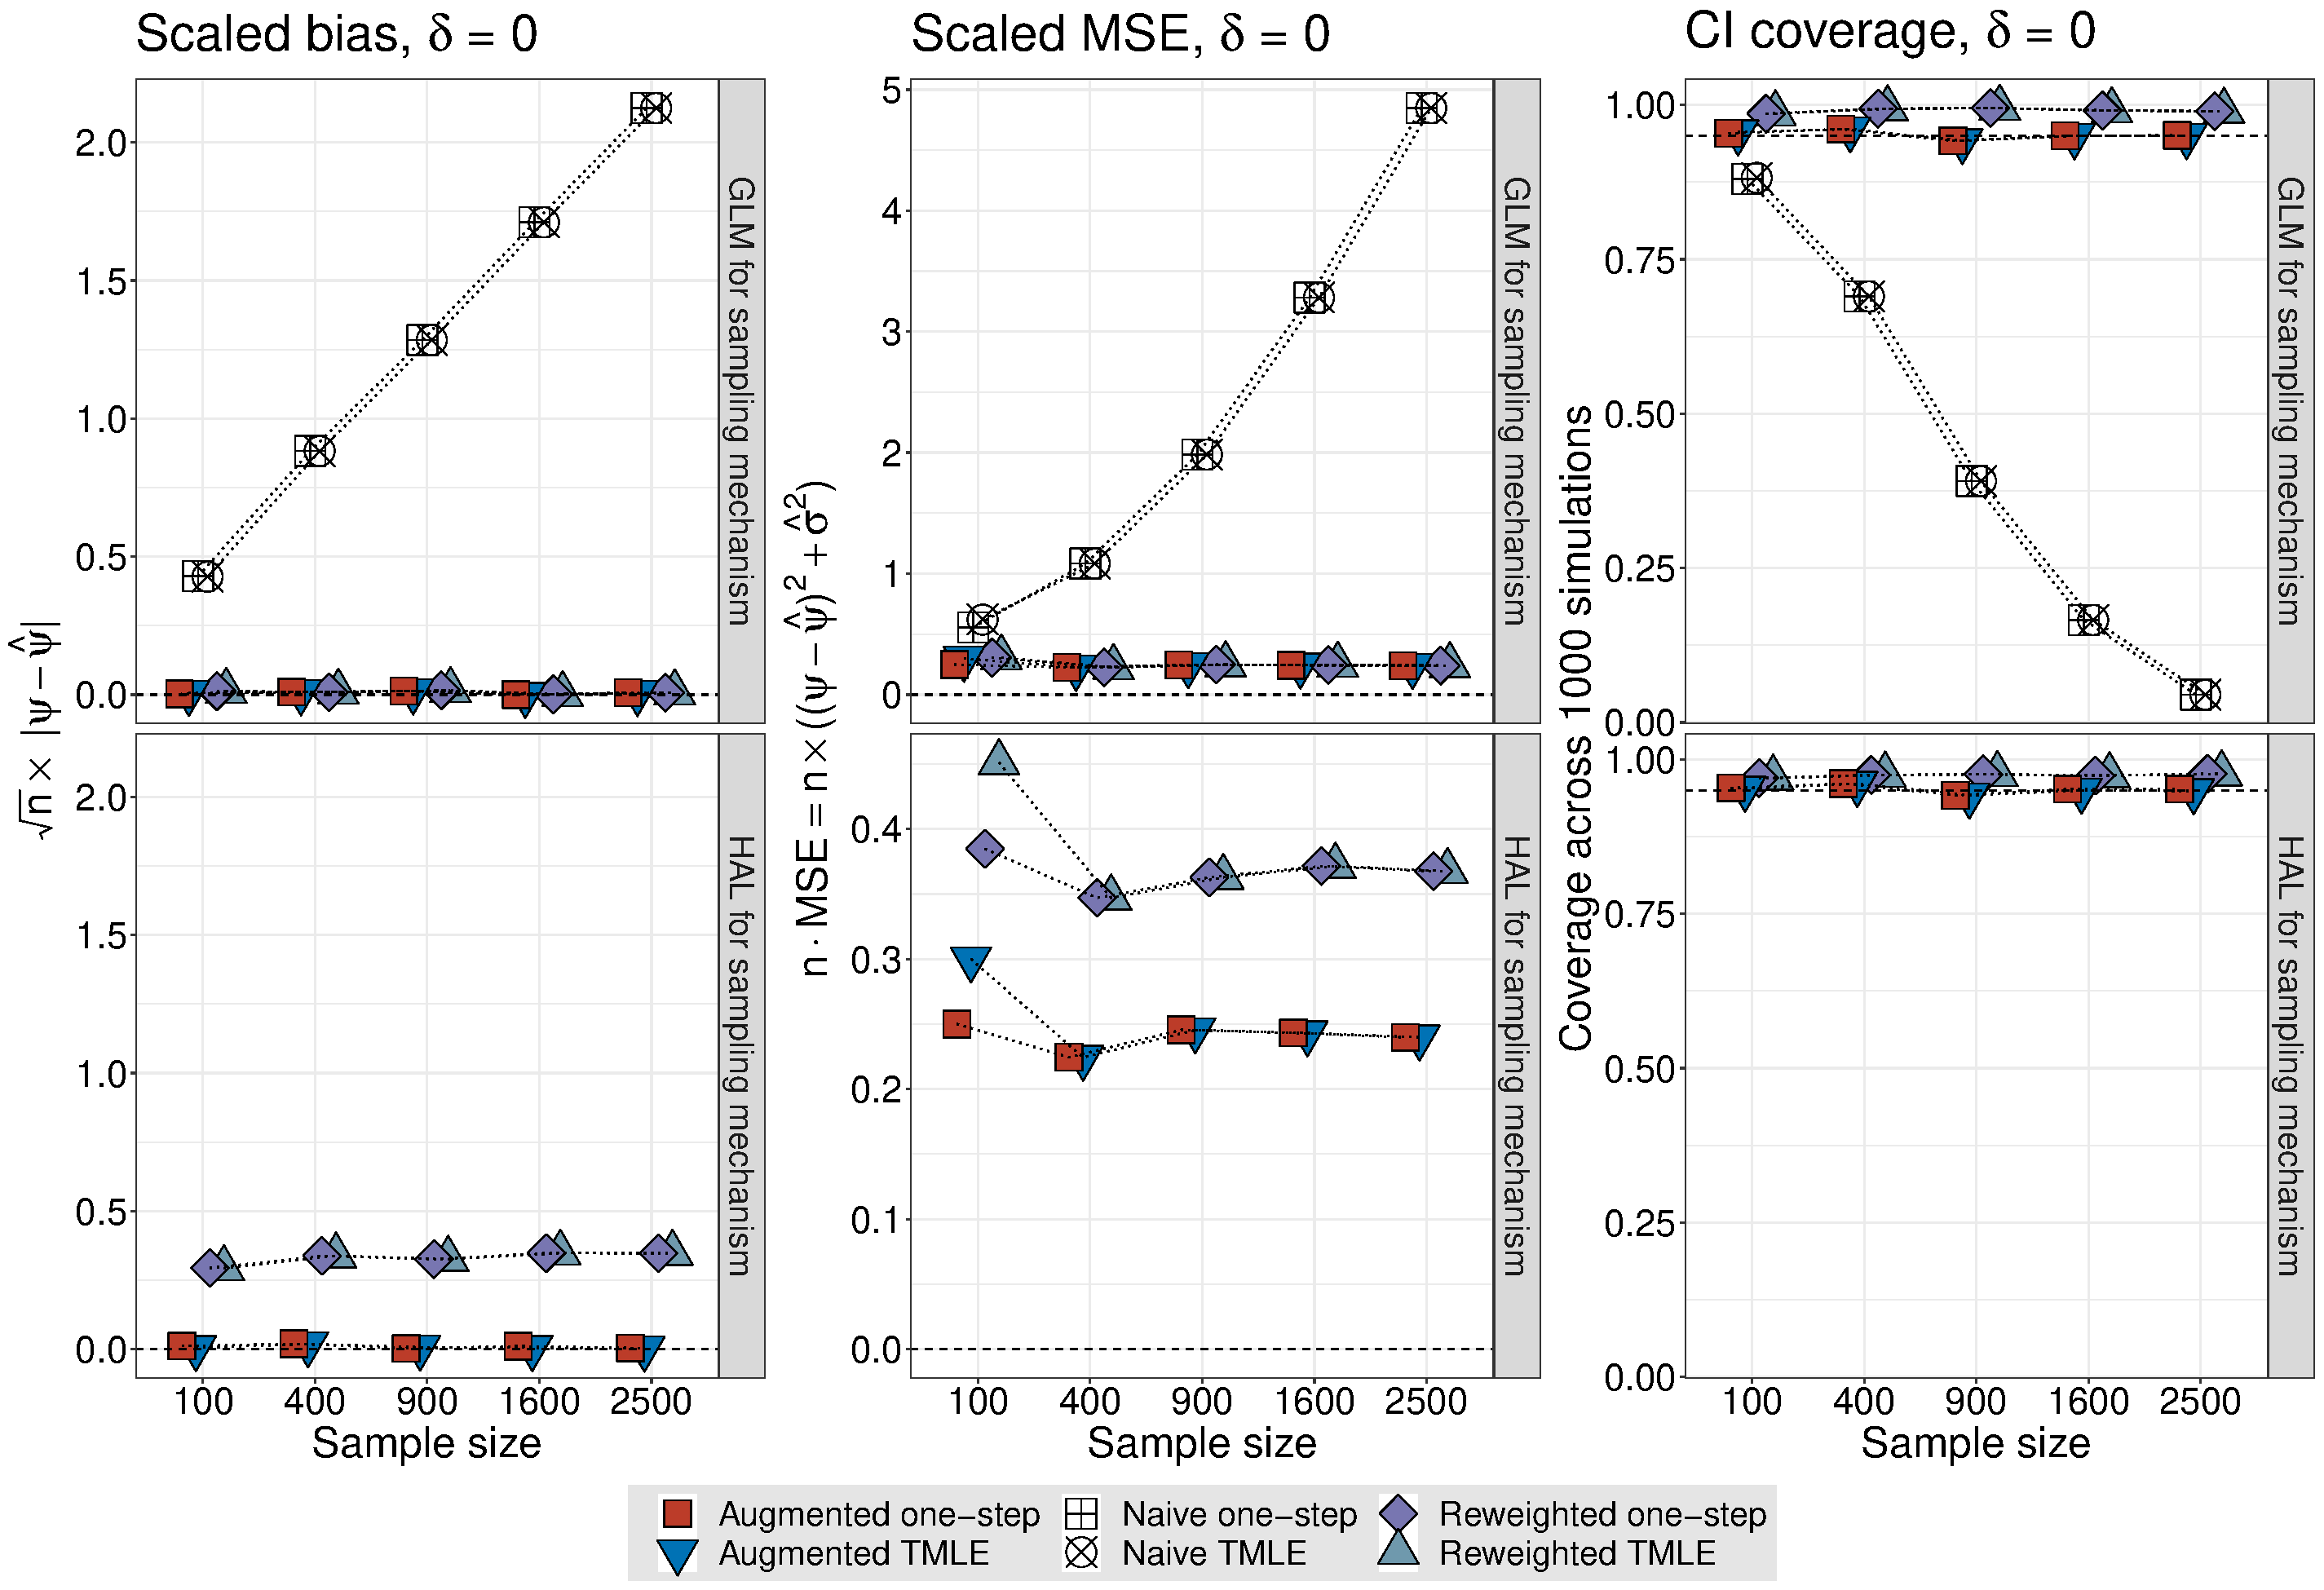
\includegraphics[scale=0.33]{simple_effect_panel_delta_null}
  \caption{Results of numerical simulations comparing six estimation strategies
  for $\psi_{0,\delta}$ for $\delta = 0$.}
  \label{fig:simple_sim_delta_noshift}
\end{figure}

\begin{figure}[H]
  \centering
  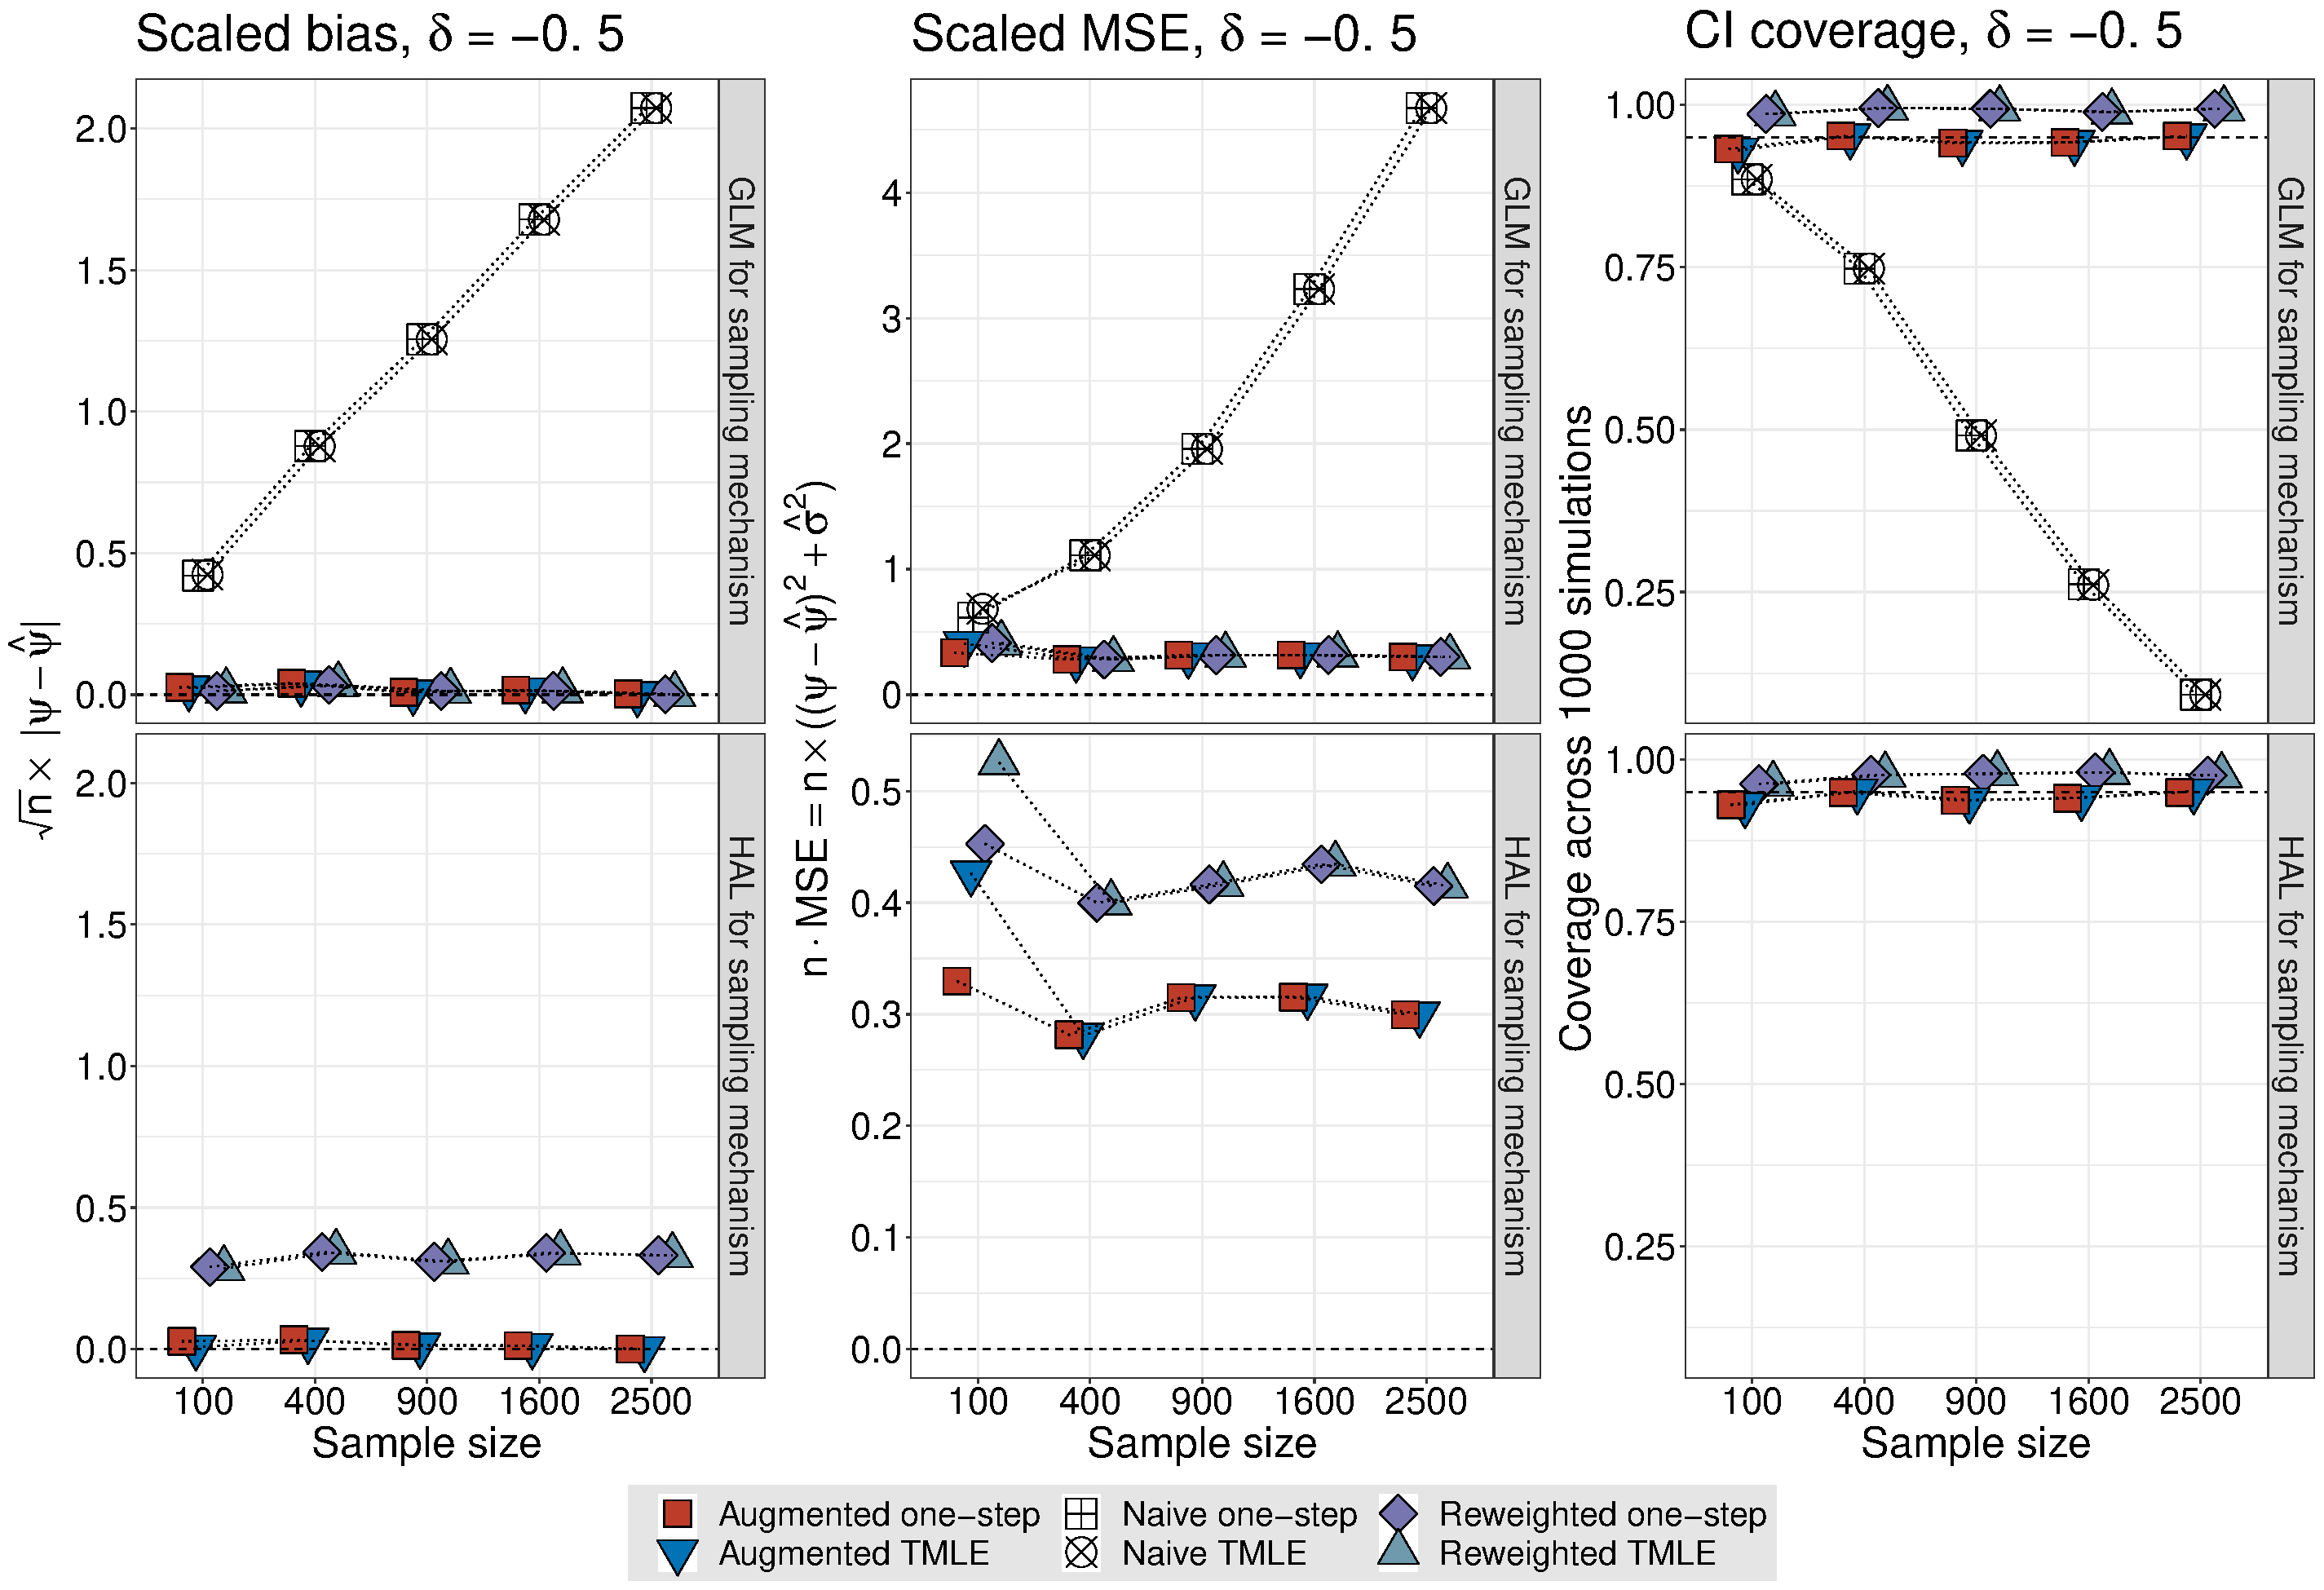
\includegraphics[scale=0.33]{simple_effect_panel_delta_downshift}
  \caption{Results of numerical simulations comparing six estimation strategies
  for $\psi_{0,\delta}$ for $\delta = -0.5$.}
  \label{fig:simple_sim_delta_downshift}
\end{figure}

Both the reweighted estimators of~\citet{rose2011targeted2sd} and our augmented
estimators display the expected level of performance when the sampling mechanism
is estimated via a correctly specified parametric model, standing out against
the performance of their unadjusted counterparts. As in the case of $\delta
= 0.5$, the reweighted estimators display coverage exceeding the desired 95\%
level, while their augmented analogs cover at exactly the nominal level. This
suggests again that the reweighted estimators exhibit an inflated variance
relative to that of our augmented estimators. The lower panel of each figure
visualizes differences in the performance of the estimators when the sampling
mechanism is estimated flexibly via HAL. These results reveal a significant
discrepancy in the performance of the reweighted and augmented estimators, with
our augmented one-step and TML estimators outperforming their reweighted
counterparts in terms of $\sqrt{n}$-bias, $n$-MSE, and coverage. In this second
case, we note that the TML estimators appear to exhibit a small degree of
estimation instability at $n = 100$, displaying larger $n$-MSE in both the
reweighted and augmented variants. We conjecture that this performance is due to
an instability induced by the targeting procedure --- in practice, this could be
ameliorated by alterations to the convergence criterion. Overall, the results of
these numerical investigations do not differ substantially from those presented
in section~\ref{sim}, establishing that our augmented estimators improve
upon alternative estimation strategies when nonparametric estimation of
$g_{0,C}$ is performed.

\subsubsection{Simulation \#2a: Comparing estimators in a scenario based on
  the HVTN 505 trial}\label{hvtn_sim}

For use in real data analysis, we examine only our augmented one-step and TML
estimators. We used the HVTN data to calibrate the following data-generating
mechanism:
\begin{align*}
  W_1 & \sim \mbox{Normal}(26.6, 5.7);
  W_2 \sim \text{Poisson}(40);
  W_3 \sim \bern(0.4);
  W_4 \sim \bern(0.3) \\
  A \mid W & \sim \mbox{Normal}(-1.37 + 0.004 W_1 + 0.015 W_2 + 0.05 W_3 +
    0.25 W_4, 0.2^2)\\
  Y \mid A, W & \sim \bern \left(\expit (-2.9 - 0.0013 W_1 - 0.0016 W_2 +
    0.0678 W_3 + 0.039 W_4 - 0.033 A) \right) \\
  C \mid Y, W & \sim
    \begin{cases}
      \bern \left(\expit (-2.45 - 0.027 W_1 + 0.012 W_2 + 0.39 W_3
      + 0.166 W_4) \right), & Y = 0 \\ 1, & Y = 1
    \end{cases} \ .
\end{align*}
Here, each of the structural equations were generated by fitting parametric
linear or logistic models for $\E[A \mid W]$, $\E[Y \mid A, W]$ and $\E[C \mid
Y = 0, W]$, the means of the CD4+ immunogenic marker, HIV-1 infection risk at
month 24, and probability of inclusion in the second-phase sample, respectively.
Meanwhile, the forms of $W_1, \ldots W_4$ were based on examination of the
empirical distributions of the relevant baseline covariates. Specifically, with
respect to the data from the HVTN 505 trial, $W_1$ mimics BMI, $W_2$ is based on
participants' age, $W_3$ is a binarized clinical behavioral risk score for HIV-1
infection, and $W_4$ behaves as the binarized race/ethnicity. For consistency
with the observed rate of HIV infection in the HVTN 505 trial, the outcome was
made to have a relatively rare event rate, with $\prob(Y = 1 \mid A, W) \approx
0.059$. We considered a setting where we observed $n = 1400$
i.i.d.~observations, approximately matching the sample size of the vaccinated
arm in HVTN 505. Estimator performance was assessed and reported by aggregating
across 1000 repetitions. Under this data-generating mechanism, the true
parameter values were approximated as $\psi_{0,\delta} = \{0.0627, 0.0617,
0.0609, 0.0598, 0.0589, \allowbreak 0.0580, 0.0571, 0.0561, 0.0554\}$ for
$\delta \in \{-2.0, -1.5, -1.0, \allowbreak -0.5, 0.0, 0.5, 1.0, 1.5, 2.0\}$,
respectively. An analogous setting, in which the effect of exposure on the
outcome was removed, yielded similar results.

The proposed estimators were constructed by using the highly adaptive lasso to
estimate the sampling mechanism $g_{n,C}$, the exposure mechanism $q_{n,A}$, the
outcome mechanism $\overline{Q}_{n,Y}$, and the pseudo-outcome regression $G_n$.
We compared the proposed one-step and TML estimators in terms of their bias,
MSE, and coverage of 95\% confidence intervals, summarizing the results in
Figure~\ref{fig:hvtn_sim_moderate}.
\begin{figure}[H]
  \centering
  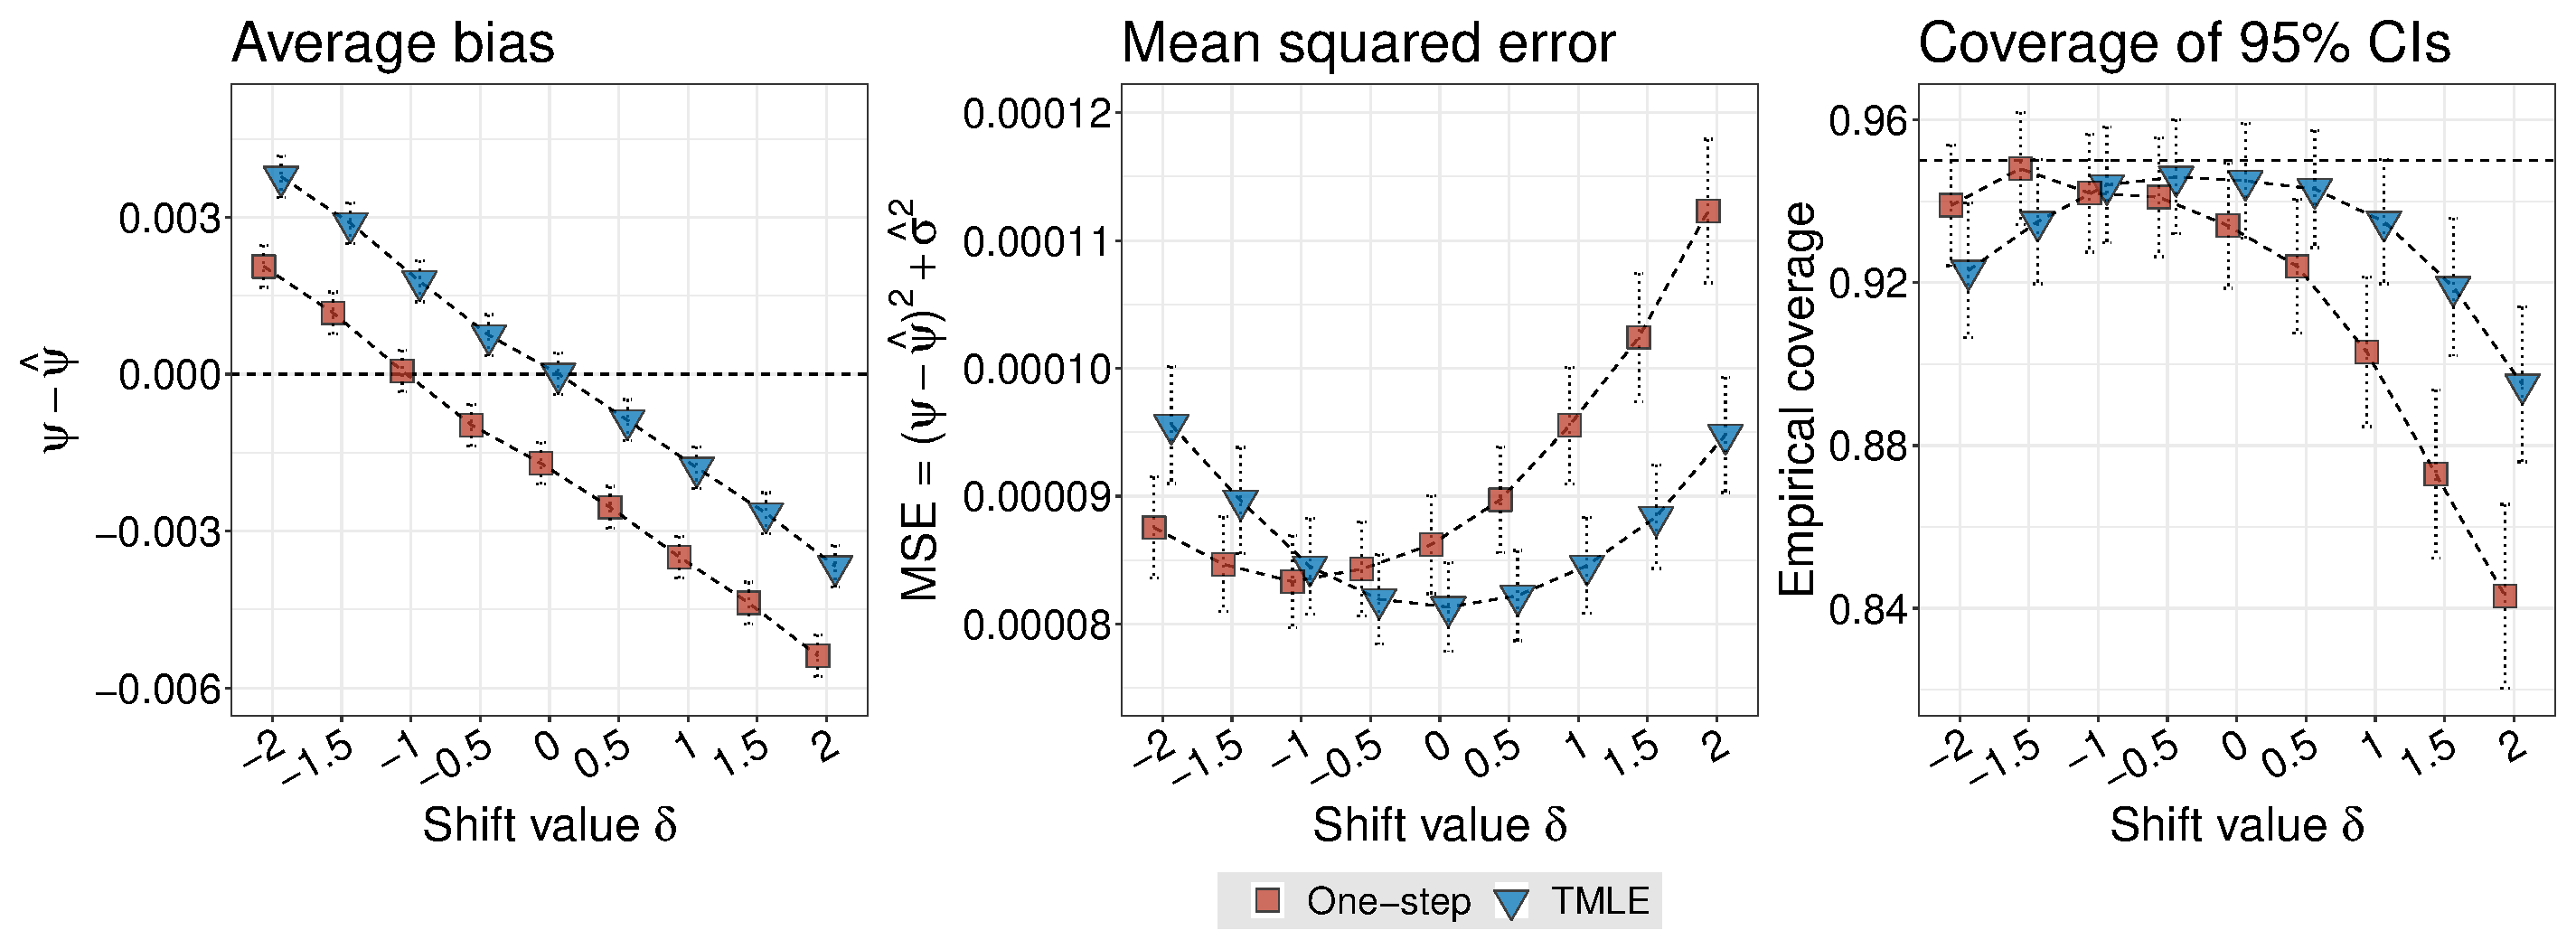
\includegraphics[scale=0.35]{hvtn505_moderate_panel}
  \caption{Results of numerical simulations comparing our two proposed
  estimators of $\psi_{0,\delta}$ for a grid of $\delta$, across 1000 Monte
  Carlo simulations at $n = 1400$.}
  \label{fig:hvtn_sim_moderate}
\end{figure}

%Primarily, the aim of this simulation study is to ascertain whether our
%augmented estimators would perform adequately in a setting similar to our
%motivating HVTN 505 trial. \db{Move up, move up} In contrast to the case of the
%simulation scheme described in section~\ref{simple_sim}, all nuisance parameters
%are estimated only via nonparametric HAL regression --- in this way, we ensure
%that the conditions of our theoretical results are satisfied. An initial
%estimator of the outcome mechanism $\overline{Q}_{n,Y}$ is based on a HAL
%classification model, while the initial estimator of the exposure mechanism
%$q_{n,A}$ is constructed via our HAL-based conditional density estimator
%(described in section~\ref{est_nuisance_param}). Just as with the augmented
%estimators featured in the lower panel of
%Figure~\ref{fig:simple_sim_delta_upshift}, the sampling mechanism $g_{n,C}$ and
%the pseudo-outcome regression $G_n$ were estimated using distinct HAL
%regressions.

Inspection of the bias and MSE indicates that both of our proposed estimators
display adequate performance, with small finite-sample bias and mean squared
error. In terms of bias, the TML estimator outperforms the one-step at $\delta
\geq -0.5$ while the one-step provides better performance at $\delta \leq -0.5$.
Given the exceedingly small scale of the bias, we conclude this to be
a particularity of this data-generating mechanism, not to be used as a guiding
principle in practice. The bias appears to dominate the MSE, with the parabolic
forms of the MSE curves having their respective minima at points at which each
of the estimators is unbiased. Here, the two estimators achieve comparable
performance at $\delta \leq 0$ but the TML estimator outperforms the one-step at
other values of $\delta$. Similarly, in terms of empirical coverage, both
estimators provide coverage near the nominal rate for $\delta \leq 0.5$ but the
performance of the TML estimator suffers less at larger $\delta$. Importantly,
we note that coverage at the nominal rate is only to be expected asymptotically
and is not guarateed by theory in the finite-sample setting presently under
consideration. From these numerical investigations, we concluded that our
augmented estimators are both well-suited to estimating $\psi_{0,\delta}$ in the
context of a re-analysis of data from the HVTN 505 trial.

\subsubsection{Simulation \#2b: Comparing estimators in a scenario like
HVTN 505, without effect of treatment}\label{sim2_supp}

To further assess the performance of our augmented estimators in a scenario like
the HVTN 505 trial, we replace the structural equation for the outcome $Y$ with
a draw from the Bernoulli distribution parameterized as $\bern (p = \expit(-2.8
- 0.0013 W_1 - 0.0016 W_2 + 0.0678 W_3 + 0.039 W_4))$ to achieve a setting in
which there is no effect of the treatment on the outcome. In this case, the
outcome process is relatively rare, with $\prob(Y = 1 \mid A, W) \approx
0.053$. The structural equations for other components of the observed data $O$
are unaltered. In this setting, the true parameter value was approximated to
be $\psi_{0,\delta} = 0.0526$ regardless of the value of $\delta$. We present
the results of assessing our augmented estimators in
Figure~\ref{fig:hvtn_sim_null}.
\begin{figure}[H]
  \centering
  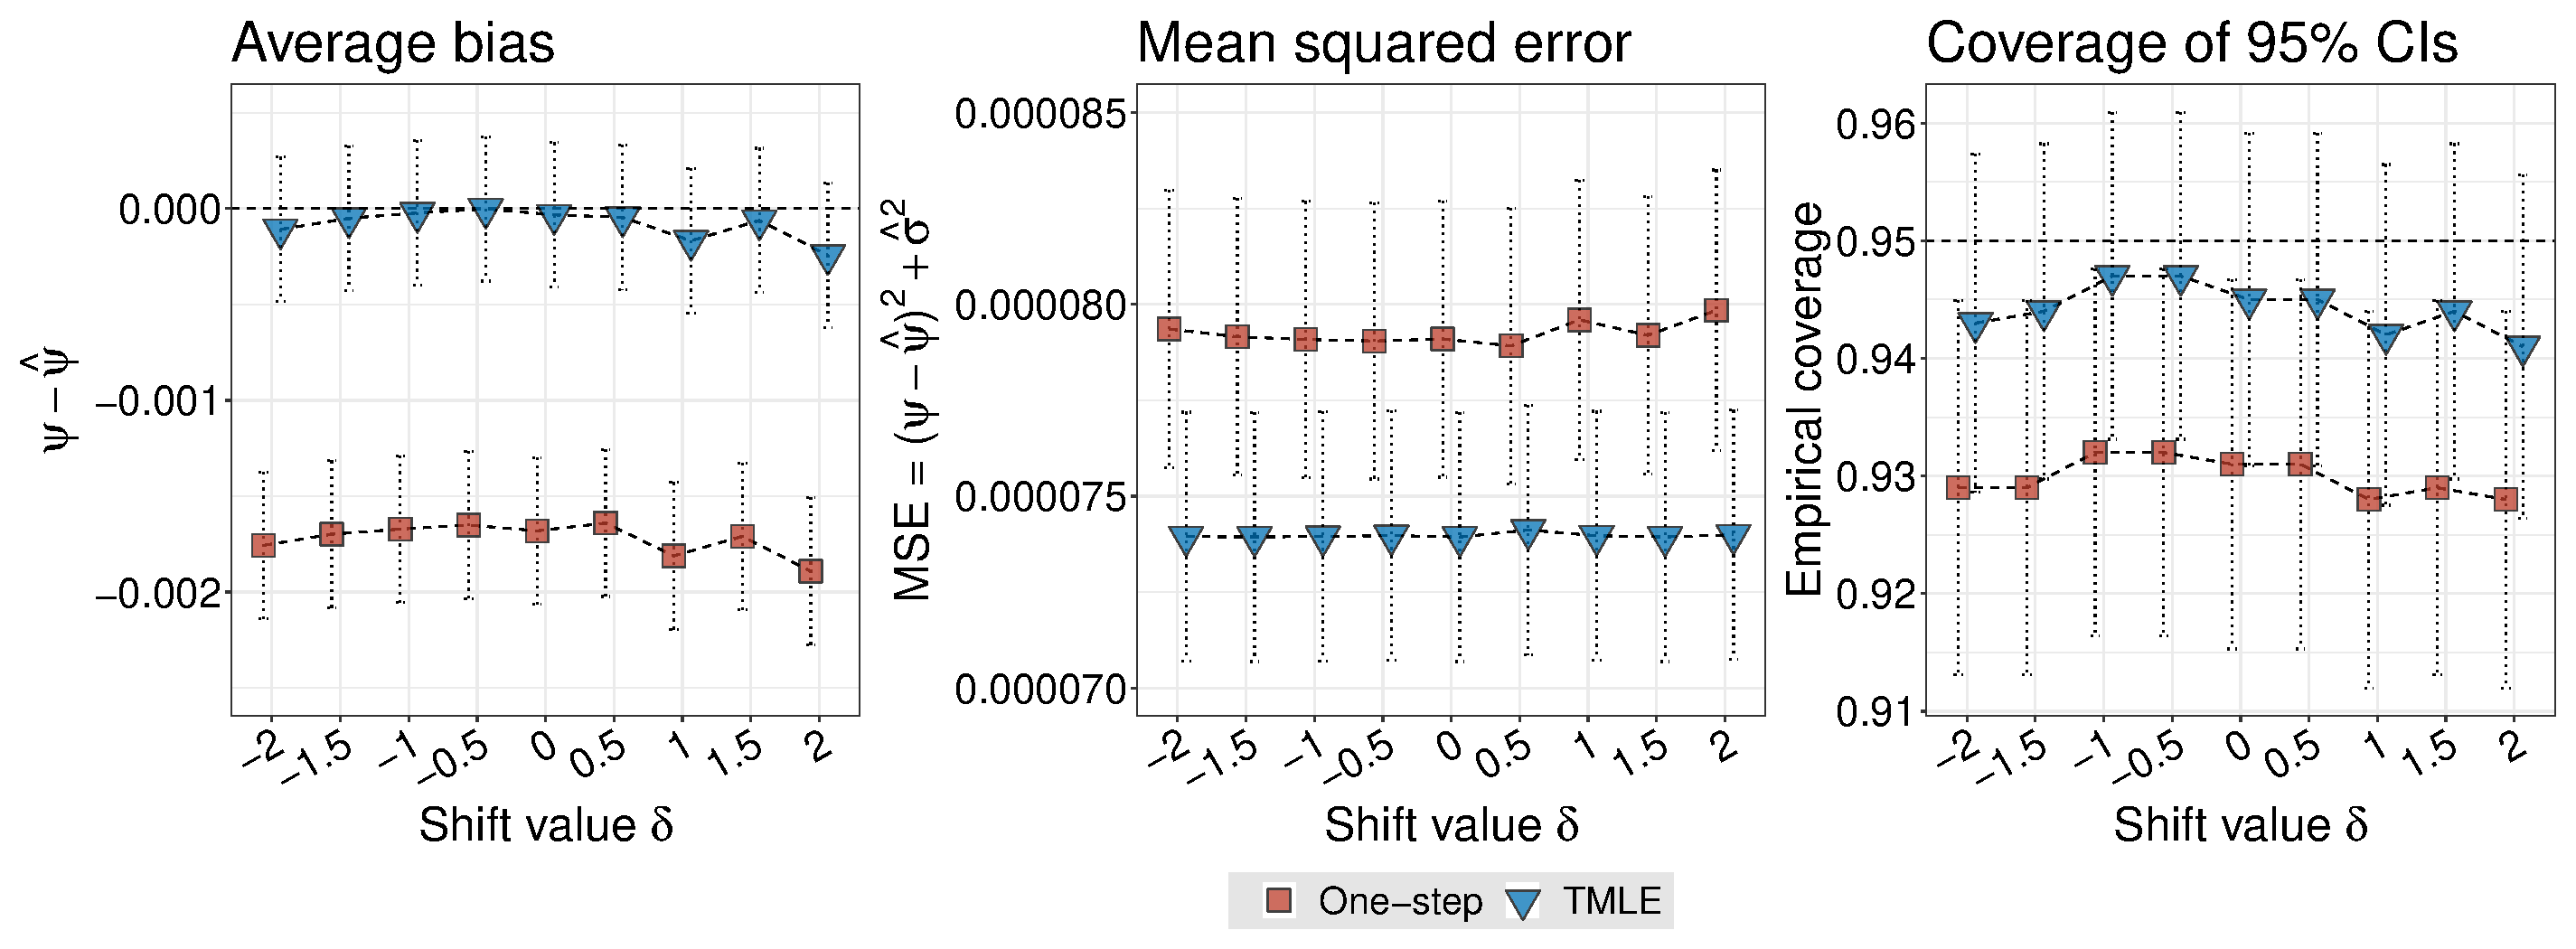
\includegraphics[scale=0.33]{hvtn505_null_panel}
  \caption{Results of numerical simulations comparing our two proposed
     estimators of $\psi_{0,\delta}$ for a grid of $\delta$, across 1000 Monte
     Carlo simulations at $n = 1400$.}
 \label{fig:hvtn_sim_null}
\end{figure}

As the ground truth of the effect of shifting the post-vaccination activity of
the CD4+ and CD8+ immunogenic markers on the risk of HIV-1 infection is unknown
in the HVTN 505 trial, we assess our estimators in this scenario so as to be
sure of there performance when no effect of treatment is present. Estimation of
all nuisance parameters is performed using exactly the same techniques outlined
previously in section~\ref{hvtn_sim}.

In terms of bias and MSE, our proposed estimators display adequate performance.
With respect to both metrics, the TML estimator outperforms the one-step
uniformly in $\delta$, though both estimators display extremely low bias and
MSE. In terms of the coverage of 95\% confidence intervals, the TML estimator
again outperforms the one-step estimator, though only very slightly. Unlike the
results presented in section~\ref{hvtn_sim}, the performance of the estimators,
in terms of all three metrics, appears stable across $\delta$, providing further
evidence that the phenomenon appearing in that numerical study was
a particularity of the effect of $A$ on $Y$ under this data-generating
mechanism. The improved performance of the TML estimator over the one-step
estimator is in line with prior demonstrations of the enhanced finite-sample
performance of TML estimators~\citep{vdl2011targeted}. As with the numerical
investigations presented in section~\ref{hvtn_sim}, these results suggest that
our augmented estimators will perform well enough to allow accurate estimation
of $\psi_{0,\delta}$ when applied to data from the HVTN 505 trial.

\subsection{Super Learner ensemble models for $\overline{Q}_{n,Y}$ in the HVTN
  505 data analysis}\label{hvtn_sl_details}

As noted in section~\ref{application}, for both the CD4+ and CD8+ analyses,
the estimated outcome mechanism $\overline{Q}_{n,Y}$ was constructed from an
ensemble model based on the super learner algorithm~\citep{vdl2007super}. The
cross-validation selector that forms the basis of the super learner has been
shown to exhibit unique theoretical guarantees, including asymptotic equivalence
to the oracle selector~\citep{vdl2004asymptotic, vdl2006cross, vdl2006oracle},
that make its use preferable over other ensemble learning approaches.

A rich library of candidate classification algorithms was considered in the
super learner ensemble model for $\overline{Q}_{n,Y}$. These included
$\ell_1$-penalized lasso regression~\citep{tibshirani1996regression,
friedman2009glmnet}; $\ell_2$-penalized ridge regression
\citep{tikhonov1977solutions,hoerl1970ridge,friedman2009glmnet}; three elastic
net regressions weighting the $\ell_1$ penalty at $\alpha \in \{0.25, 0.50,
0.75\}$ and the $\ell_2$ penaly at
$(1-\alpha)$~\citep{zou2003regression,friedman2009glmnet}; random
forests~\citep{breiman2001random} with 50, 100, and 500 trees based on its
implementation in the \texttt{ranger} \texttt{R}
package~\citep{wright2017ranger}; extreme gradient boosted trees with 20, 50,
100, and 300 fitting iterations~\citep{chen2016xgboost}; multivariate adaptive
polynomial spline regression~\citep{kooperberg1997polychotomous,stone1994use};
multivariate adaptive regression splines~\citep{friedman1991multivariate};
generalized linear models with Bayesian priors on parameters; a multilayer
perceptron~\citep{rosenblatt1961principles}; and the highly adaptive
lasso~\citep{vdl2017generally,benkeser2016highly,coyle2019hal9001}. The
implementation of the super learner algorithm in the \texttt{sl3} \texttt{R}
package~\citep{coyle2020sl3} was used, and weights assigned to each learning
algorithm by the super learner are given in Tables~\ref{tab:cd4_sl_coefs}
and~\ref{tab:cd8_sl_coefs} for the CD4+ and CD8+ analyses, respectively.

\begin{table}[H]
\caption{\label{tab:cd4_sl_coefs} Weights and risk estimates assigned to each
  individual learning algorithm in the ensemble model for $\overline{Q}_{n,Y}$
  used in the reported re-analysis of the CD4+ immunogenic marker.}
\centering
\begin{tabular}[t]{l|r|r|r|r}
\hline
Learner & Weight & Min. Fold Risk & Mean CV-Risk & Max. Fold Risk\\
\hline
Ridge ($\ell_2$ penalized) & 0.147 & 0.015 & 0.036 & 0.052\\
\hline
Lasso ($\ell_1$ penalized) & 0.000 & 0.015 & 0.036 & 0.052\\
\hline
Elastic net ($\alpha = 0.25$) & 0.116 & 0.015 & 0.036 & 0.051\\
\hline
Elastic net ($\alpha = 0.50$) & 0.000 & 0.015 & 0.036 & 0.051\\
\hline
Elastic net ($\alpha = 0.75$) & 0.181 & 0.015 & 0.036 & 0.051\\
\hline
Random forest (50 trees) & 0.000 & 0.062 & 0.097 & 0.173\\
\hline
Random forest (100 trees) & 0.000 & 0.050 & 0.093 & 0.153\\
\hline
Random forest (500 trees) & 0.000 & 0.061 & 0.093 & 0.158\\
\hline
xgboost(20 iterations) & 0.000 & 0.012 & 0.072 & 0.165\\
\hline
xgboost(50 iterations) & 0.000 & 0.012 & 0.080 & 0.181\\
\hline
xgboost(100 iterations) & 0.010 & 0.013 & 0.088 & 0.192\\
\hline
xgboost(500 iterations) & 0.000 & 0.012 & 0.098 & 0.204\\
\hline
Highly adaptive lasso (default) & 0.014 & 0.064 & 0.074 & 0.084\\
\hline
Highly adaptive lasso (custom) & 0.000 & 0.066 & 0.075 & 0.084\\
\hline
Multivariate adaptive regression splines & 0.000 & 0.050 & 0.086 & 0.131\\
\hline
Polynomial spline regression & 0.208 & 0.015 & 0.036 & 0.053\\
\hline
Multilayer perceptron network & 0.000 & 0.015 & 0.037 & 0.055\\
\hline
GLM with Bayesian priors & 0.323 & 0.015 & 0.036 & 0.051\\
\hline
Super Learner & 1.000 & --- & --- & ---\\
\hline
\end{tabular}
\end{table}

In the super learner ensemble model for the outcome regression in the CD4+
analysis, the three best learning algorithms were a GLM with Bayesian priors on
parameter estimates, a polynomial spline regression model, and an elastic net
regression model that favored the $\ell_1$ (lasso) penalty over the $\ell_2$
(ridge) penalty. Another variant of elastic net regression, which favored the
$\ell_2$ penalty over the $\ell_1$ penalty, and ridge regression were also given
nontrivial weights in the ensemble model. A variant of extreme gradient boosting
and the highly adaptive lasso received low weights, while all other candidate
algorithms in the library were assigned weights of zero.

\begin{table}[H]
\caption{\label{tab:cd8_sl_coefs} Weights and risk estimates assigned to each
  individual learning algorithm in the ensemble model for $\overline{Q}_{n,Y}$
  used in the reported re-analysis of the CD8+ immunogenic marker.}
\centering
\begin{tabular}[t]{l|r|r|r|r}
\hline
Learner & Weight & Min. Fold Risk & Mean CV-Risk & Max. Fold Risk\\
\hline
Ridge ($\ell_2$ penalized) & 0.161 & 0.013 & 0.037 & 0.075\\
\hline
Lasso ($\ell_1$ penalized) & 0.161 & 0.011 & 0.037 & 0.075\\
\hline
Elastic net ($\alpha = 0.25$) & 0.003 & 0.012 & 0.037 & 0.075\\
\hline
Elastic net ($\alpha = 0.50$) & 0.000 & 0.014 & 0.037 & 0.076\\
\hline
Elastic net ($\alpha = 0.75$) & 0.131 & 0.014 & 0.037 & 0.074\\
\hline
Random forest (50 trees) & 0.090 & 0.053 & 0.088 & 0.129\\
\hline
Random forest (100 trees) & 0.055 & 0.048 & 0.089 & 0.136\\
\hline
Random forest (500 trees) & 0.119 & 0.049 & 0.088 & 0.127\\
\hline
xgboost(20 iterations) & 0.000 & 0.043 & 0.064 & 0.112\\
\hline
xgboost(50 iterations) & 0.000 & 0.036 & 0.074 & 0.128\\
\hline
xgboost (100 iterations & 0.000 & 0.031 & 0.076 & 0.134\\
\hline
xgboost (300 iterations) & 0.000 & 0.029 & 0.086 & 0.146\\
\hline
Highly adaptive lasso (default) & 0.000 & 0.046 & 0.078 & 0.115\\
\hline
Highly adaptive lasso (custom) & 0.000 & 0.044 & 0.078 & 0.132\\
\hline
Multivariate adaptive regression splines & 0.000 & 0.029 & 0.100 & 0.159\\
\hline
Polynomial spline regression & 0.000 & 0.015 & 0.040 & 0.080\\
\hline
Multilayer perceptron network & 0.067 & 0.007 & 0.040 & 0.085\\
\hline
GLM with Bayesian priors & 0.214 & 0.016 & 0.037 & 0.073\\
\hline
Super Learner & 1.000 & --- & --- & ---\\
\hline
\end{tabular}
\end{table}

In the CD8+ analysis, the three best learning algorithms, chosen by the super
learner ensemble model for the outcome regression, were a GLM with Bayesian
priors on parameter estimates, ridge regression, and lasso regression. Other
algorithms that were assigned nontrivial weights included an elastic net
regression model that favored the $\ell_1$ (lasso) penalty over the $\ell_2$
(ridge) penalty and a random forest with 500 trees. A variant of elastic net
regression, random forests with 50 and 100 trees, and a multilayer perceptron
all received low weights, while all other candidate algorithms in the library
were assigned weights of zero.
